\chapter{Data Quality Analysis} \label{ch:data}

Beginning in March of 2012, the LHC began seven months of pp collisions at $\sqrt{s} = \,$ 8 TeV. During the seven months of data taking, the ALICE Experiment was recording data almost 60\% of the time, Figure \ref{fig:RunEffer}, with stable beams.

\begin{figure}[h]
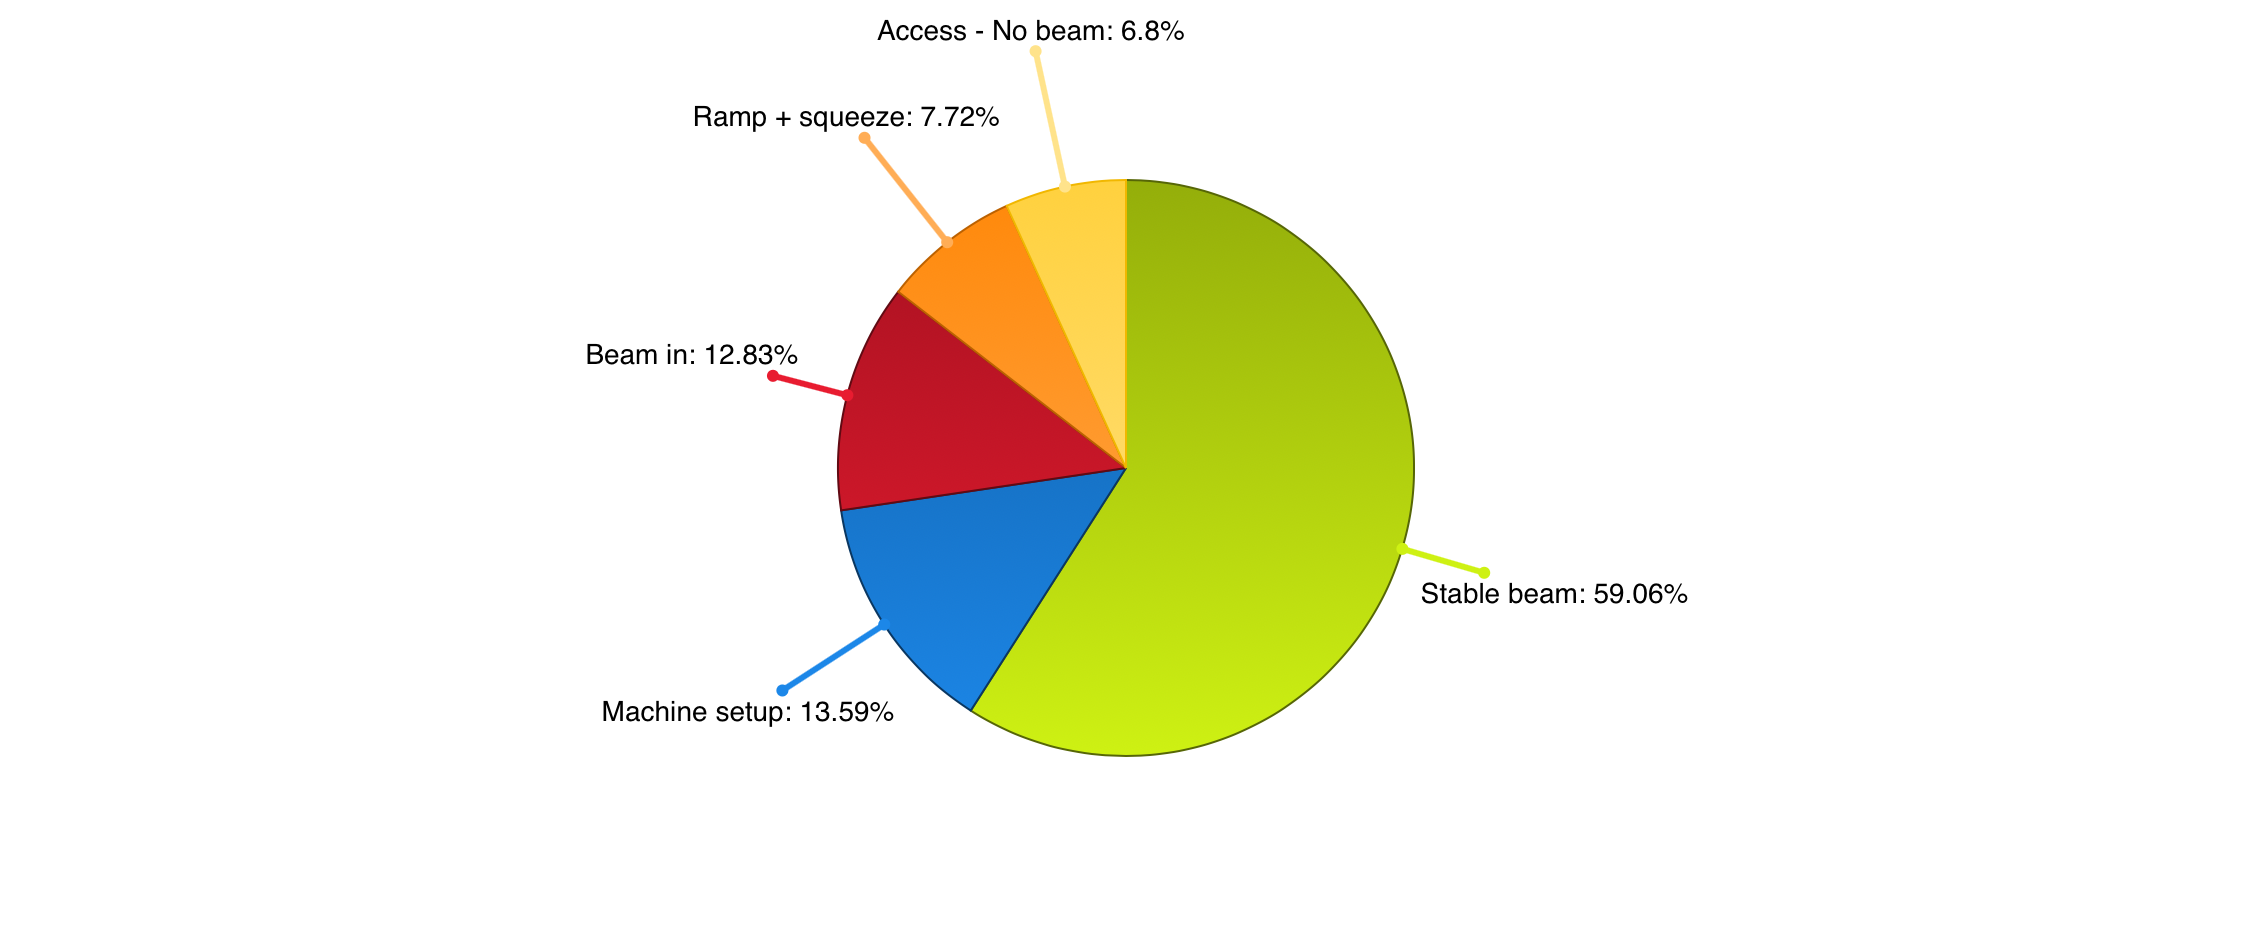
\includegraphics[width=17cm]{8TeVRunefficency}
\centering
\caption{LHC state during the 8 TeV run. }
\label{fig:RunEffer}
\end{figure}


Almost 200 million events were recorded by ALICE that satisfied the Min Bias trigger.  The pp Min Bias trigger is satisfied with at least one hit recorded in the SPD or V0.  The 8 TeV data set also recorded high-$p_{T}$ events using the EMCal triggered data, which in the case of the Gamma trigger was set at 5 GeV.  


ALICE is a state-of-the-art experiment with excellent tracking and particle identification capabilities, as discussed in Chapter \ref{ch:alice}.  However, just like any real world experiment, it contains a number of inefficiencies and imperfections.  This means that the data collected during the 8 TeV pp collisions must be examined and any inaccuracies in the data must be removed before any conclusions may be reached.  Data may be compromised at either the event-level, the experiment erroneously recorded something as an event, or at the constituent-level, one of the subdetectors mismeasured a feature of a particle.  The remainder of this chapter focuses on the corrections and quality assurance performed on the 8 TeV data.






\subsubsection{Event Selection}

During the 8 TeV data collection period, approximately 180 million Min Bias events were recorded, as summarized in table 5.1.  These events were separated into periods, which dictate the particular beam and detector configurations used during the data taking.  The 8 TeV data was broken into 7 periods, which werefurther broken into runs.  Runs represent an uninterrupted period of time during which the ALICE experiment is recording data. A run can be as short as 5 minutes or as long as 10 hours.  Runs were separated into `good' runs when both the TPC and EMCal were fully operational, `semi-good runs when a sector of the TPC was turned off but not around the region below the EMCal, and `bad' runs when a portion of the TPC was turned off directly below the EMCal or something else critically compromised the data.  This analysis only incorporated good and semi-good runs.

\begin{table}[hb]
\label{tab:RunSummary}
\begin{center}
\caption{2012 8 TeV data taking period.}
\begin{tabular}[b]{|c|c|c|}
	\hline
	Period & \# of runs & \# of Min Bias events \\ \hline
	LHC12c & 89 & $\sim \,$24 M \\ \hline
	LHC12d & 140 & $\sim \,$62 M \\ \hline
	LHC12e & 5 & $\sim \,$2 M \\ \hline
	LHC12f & 56 & $\sim \,$15 M \\ \hline
	LHC12g & 8 & $\sim \,$0.4 M \\ \hline
	LHC12h & 159 & $\sim \,$75 M \\ \hline
	LHC12i & 40 & $\sim \,$3 M \\ \hline
	Total & 497 & $\sim \,$181 M \\ \hline

\end{tabular}
\end{center}

\end{table}

Approximately 15\% of the data sampled was unusable due to malfunctions in TPC chambers, EMCal super modules, or the electronics of the EMCal or TPC.  The LHC12f  and LHC12g EMCal triggered data is not used in this analysis due to the trigger threshold being varied from the other periods.  Besides the bad runs excluded from each of the periods due to detector inefficiencies and the triggered LHC12f and LHC12g data, the rest of the 8 TeV data was used to generate the jet cross-sections in this thesis.  The LHC reported the integrated luminosity as $\mathscr{L}_{int} = 8.95 \, pb^{-1}$ during this data taking\cite{ALICE-PUBLIC-2017-002}.

\subsubsection{Monte Carlo Anchored Data}
Two Monte Carlo data sets, LHC15l2a1 and LHC15l2a2, which included a full GEANT4 simulation of the ALICE detector were produced by the ALICE collaboration and used for the Monte Carlo corrections in this analysis.   LHC15l2a1 uses a Pythia particle-level simulation embedded, or anchored, in a ALICE GEANT4 simulation with about 17 million Min Bias generated events.  LHC15l2a2 uses a PHOjet anchored data set consisting of about 21 million Min Bias triggered events.  Neither of these data driven Monte Carlos modeled the EMCal triggers.  Monte Carlo corrections of the EMCal triggered data suffered due to the lack of any simulations of the trigger and this is discussed in more detail later in this chapter.

\subsubsection{Event Selection Criteria}
For an event to be selected into a physics analysis it must pass a number of quality control tests.  For example, the LHC must be in a state of stable beams, cosmic rays must be excluded by only accepting tracks that originate from a vertex inside the detector, and the relevant detectors for a given analysis must be functioning as intended.  A number of these quality assurance, QA, were performed at the event level to exclude bad data, this thesis required the following criteria:

\begin{itemize}
  \item The event has a primary vertex reconstructed.
  \item The primary vertex occurs within a 10 cm window of the primary interaction point.
  \item The vertex resolution must be below 0.25 cm.
  \item The event passes basic pile-up checks based on the V0 and T0 signals.
\end{itemize}


A summary of the rejection reasons for an event are shown in Figure \ref{fig:eventqa}.  Most of the rejected events were excluded due to the event not satisfying the vertex requirements.

\begin{figure}[h]
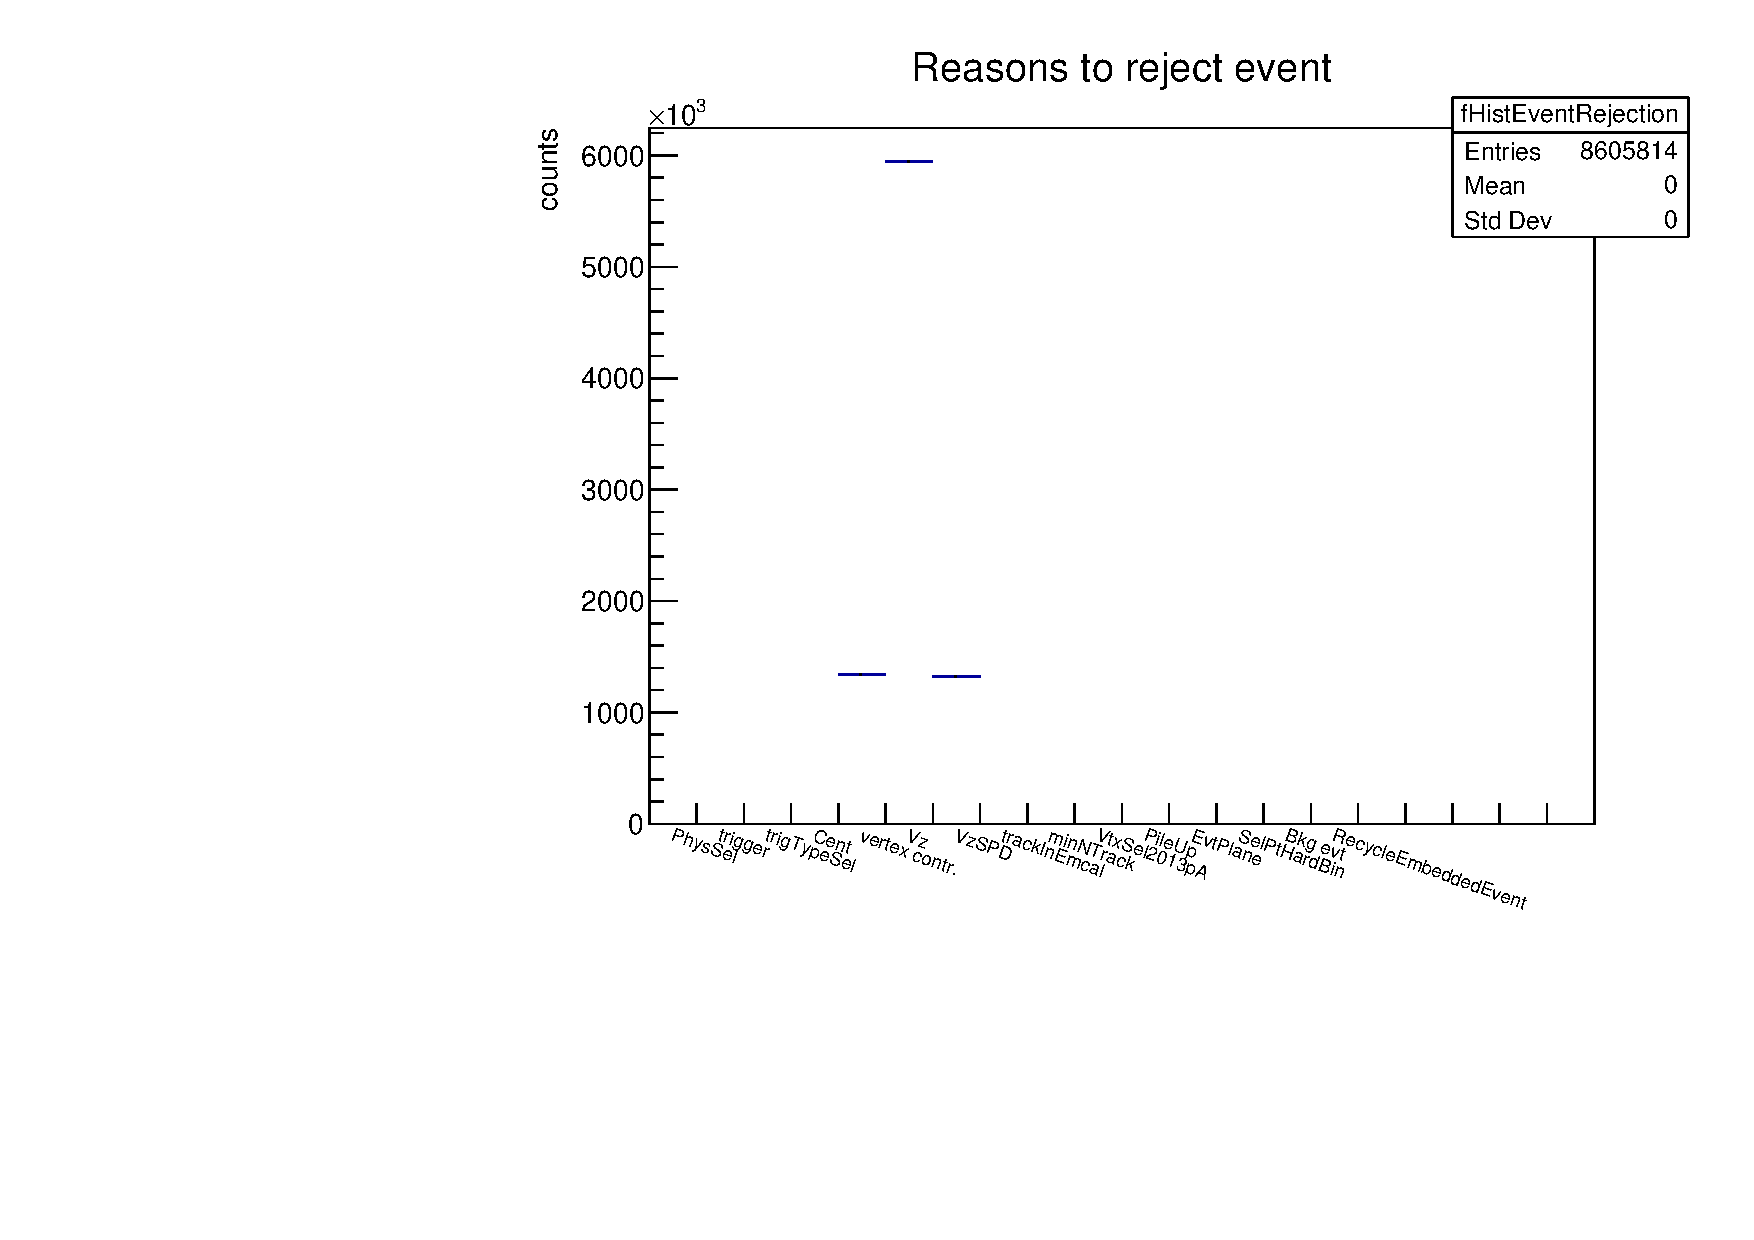
\includegraphics[width=8.5cm]{RejectionReasons}
\centering
\caption{Min Bias event rejection summary.}
\label{fig:eventqa}
\end{figure}

\begin{figure}[h]
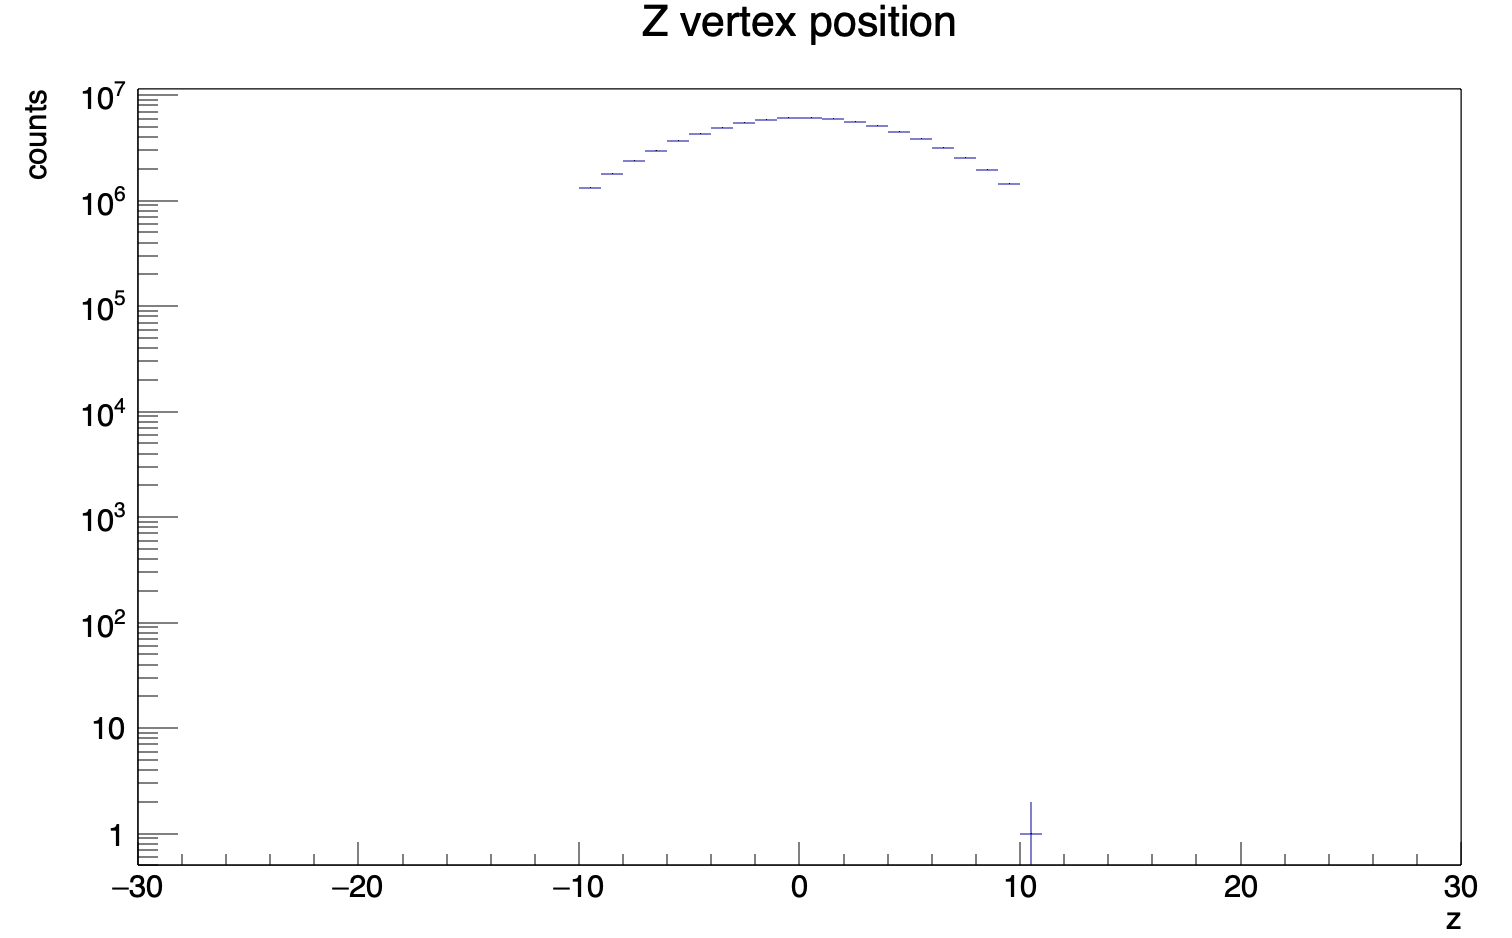
\includegraphics[width=8.5cm]{zvertex}
\centering
\caption{Vertex displacement from primary interaction point for accepted Min Bias events.}
\label{fig:vertrec}
\end{figure}


Figure \ref{fig:vertrec} shows the reconstructed vertex for the accepted Min Bias events after the QA was performed.  We see that the vertex distribution peaks at the primary interaction point as expected and that the distribution is well defined.  It should also be noted that a similar set of event QA was implemented to the EMCal triggered data and that the results were consistent with the Min Bias data.




\section{Cluster Selection}
Corrections were performed on EMCal cells including the removal of hot and dead towers (bad channels) based on the average occupancy and energy of the towers, calibrations to cell timing caused by the physical layout of the EMCal (such as differences in cabling length), and an energy calibration based on the $\pi^{0}$ mass.  After these corrections were applied, the towers were grouped together into clusters using the v2 algorithm.  The v2 algorithm has a minimum tower seed, $E_{seed} = \,$ 300 MeV, after which all adjacent towers with a minimum energy, $E_{cell} \geq \,$ 100 MeV, are iteratively added until a local minimum is reached.  The cluster energy is the sum of the seed and grouped neighbor tower energies.  Figure \ref{fig:badchannel} shows a bad channel map after removing the hot and dead towers from a typical run.  The $\phi$ distribution is segmented into 5 parts representing the five super modules of the EMCal.

\begin{figure}[h]
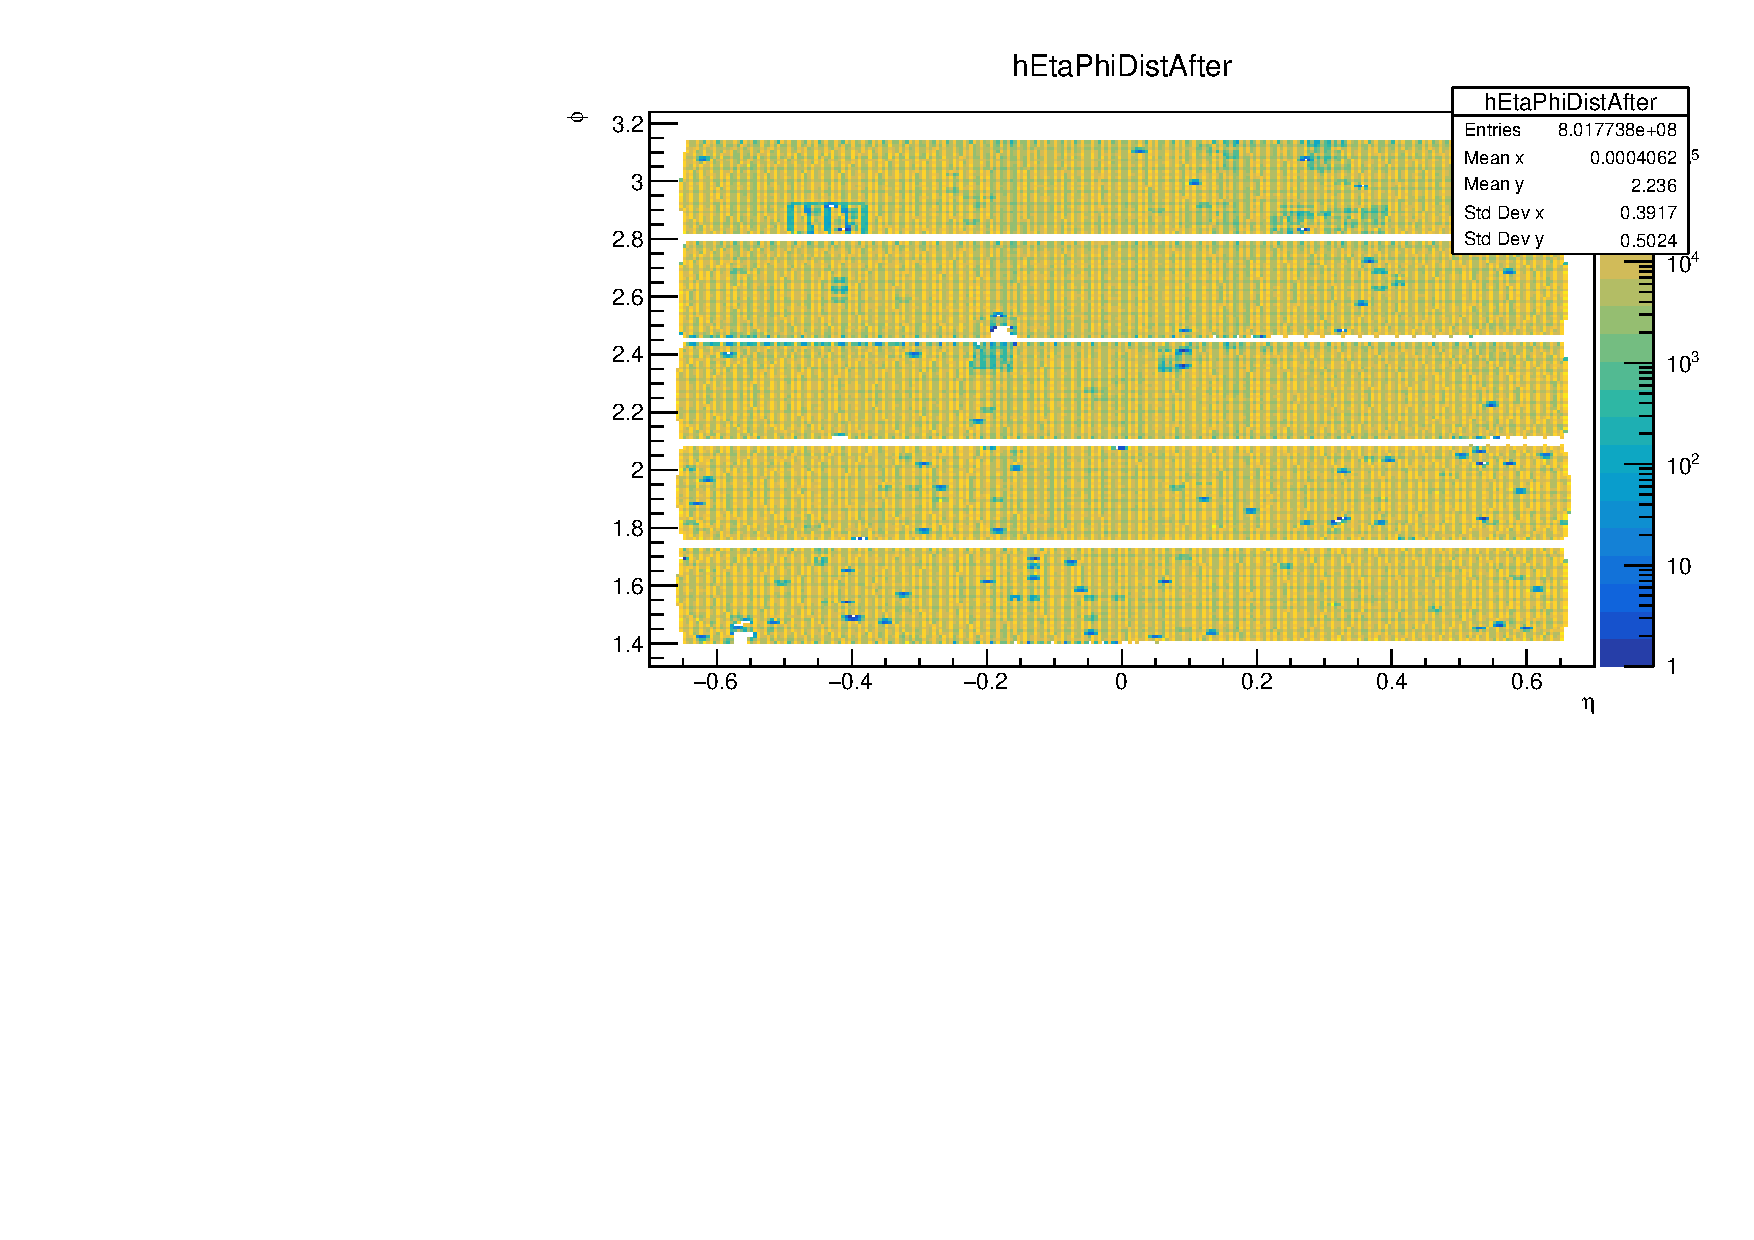
\includegraphics[width=14cm]{BadChannelMap}
\centering
\caption{EMCal cell occupancy after bad channels removed.}
\label{fig:badchannel}
\end{figure}

After the cells are clustered together the clusters are corrected for exotics.  This correction was performed by cutting all clusters with a $F_{cross} \geq \,$ 0.97, where

\begin{equation}
F_{cross} = 1 - \frac{ E_{cross} }{ E_{cell} },
\label{eq:Fcross}
\end{equation}

\noindent
where $E_{cross}$ is the sum of the four cells sharing a full edge with the leading cell and $E_{cell}$ is the center pixels energy.  The main source of exotic clusters in the EMCal is most often due to a hadron hitting the Avalanche Photodiode (APD) in a tower.  This will concentrate the energy of the cluster into a single tower while the adjacent towers will contain only a small fraction of the cluster energy.  The clusters were removed before jet finding occurred as they are an artifact of the detector performance.

The EMCal is optimized to measure the energy of electrons and photons as they tend to fully shower inside the EMCal structure.  Hadrons are detected by the EMCal, but will only shower a fraction of their intrinsic energy.  A hadronic correction was performed in order to account for this missing energy due to the partial hadron shower.  Charged tracks from the outer layer of the TPC were propagated to the EMCal, by fitting the trajectory of the track to a curve, and the of the clusters and tracks were matched together geometrically.  Figure \ref{fig:EMChadetaphi} shows the distance between the centroid of a cluster in the EMCal and the nearest track propagated from the TPC.  Hadrons are identified by requiring the matched distance to be, $\sqrt{ \Delta\phi^{2} + \Delta\eta^{2} } \leq \,$ 0.015, which is within one EMCal tower distance.

\begin{figure}[h]
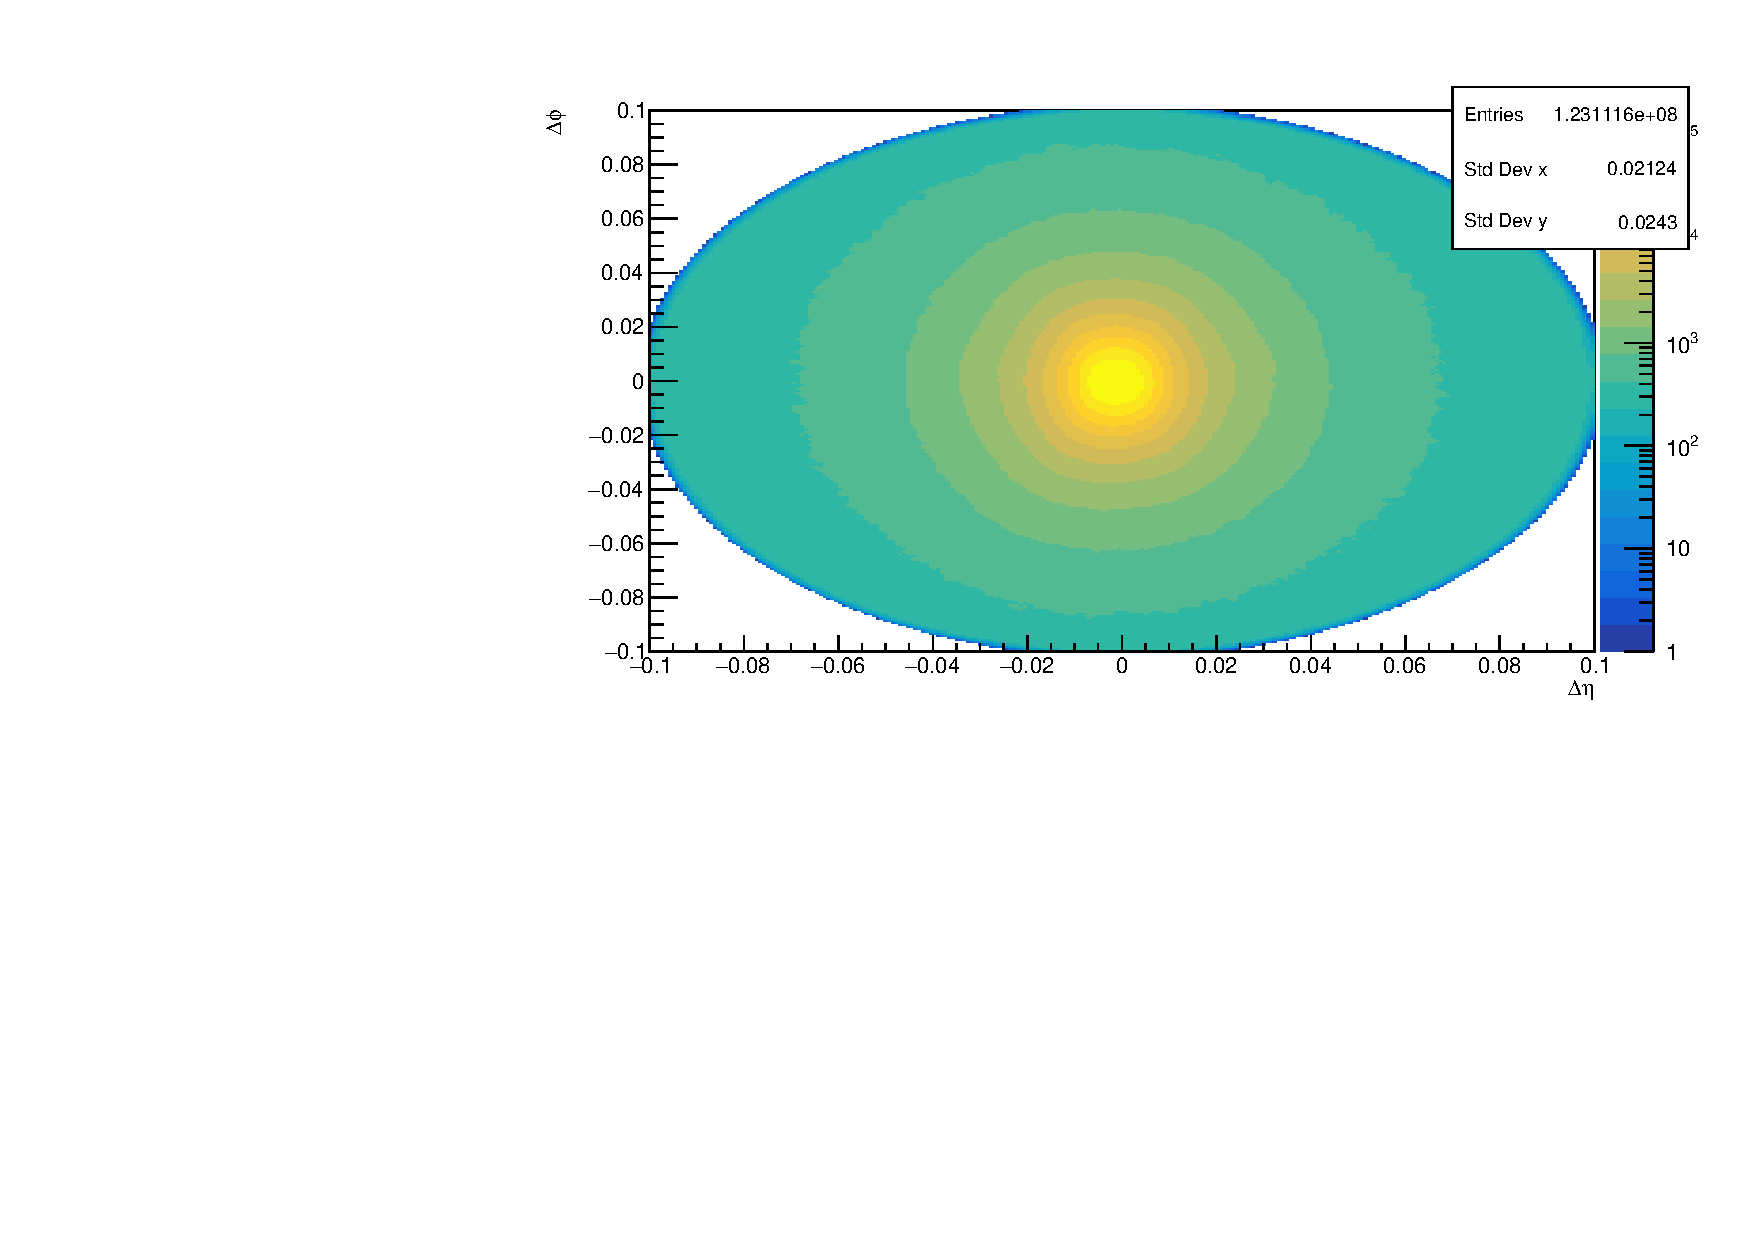
\includegraphics[width=12cm]{hadronetaphi}
\centering
\caption{Matched track-cluster distance.}
\label{fig:EMChadetaphi}
\end{figure}

\noindent
Corrections for the double counting from hadrons is based on correcting the EMCal cluster energy by a weight function,

\begin{equation}
E_{corr} = E_{clust} - f_{sub} \times \sum p ,
\label{eq:HadCorr}
\end{equation}

\noindent
where $\sum p$ is the magnitude of the 3-momentum of the hadron and $f_{sub} = 1$ is the nominal value for the weight.  If $E_{corr} \leq 0$ the cluster was removed, this may be caused by cluster pile-up and only accounted for a small fraction of the clusters.  In order for a cluster to be accepted $E_{corr} \geq \,$ 300 MeV was required, because a minimum ionizing particle (MIP) will on average deposit 280 MeV in the EMCal.  

A final cut was performed on the cluster timing, obtained from the T0, the time of arrival for a particle is shown on the y-axis of Figure \ref{fig:EMCaltime}.  

\begin{figure}[!h]
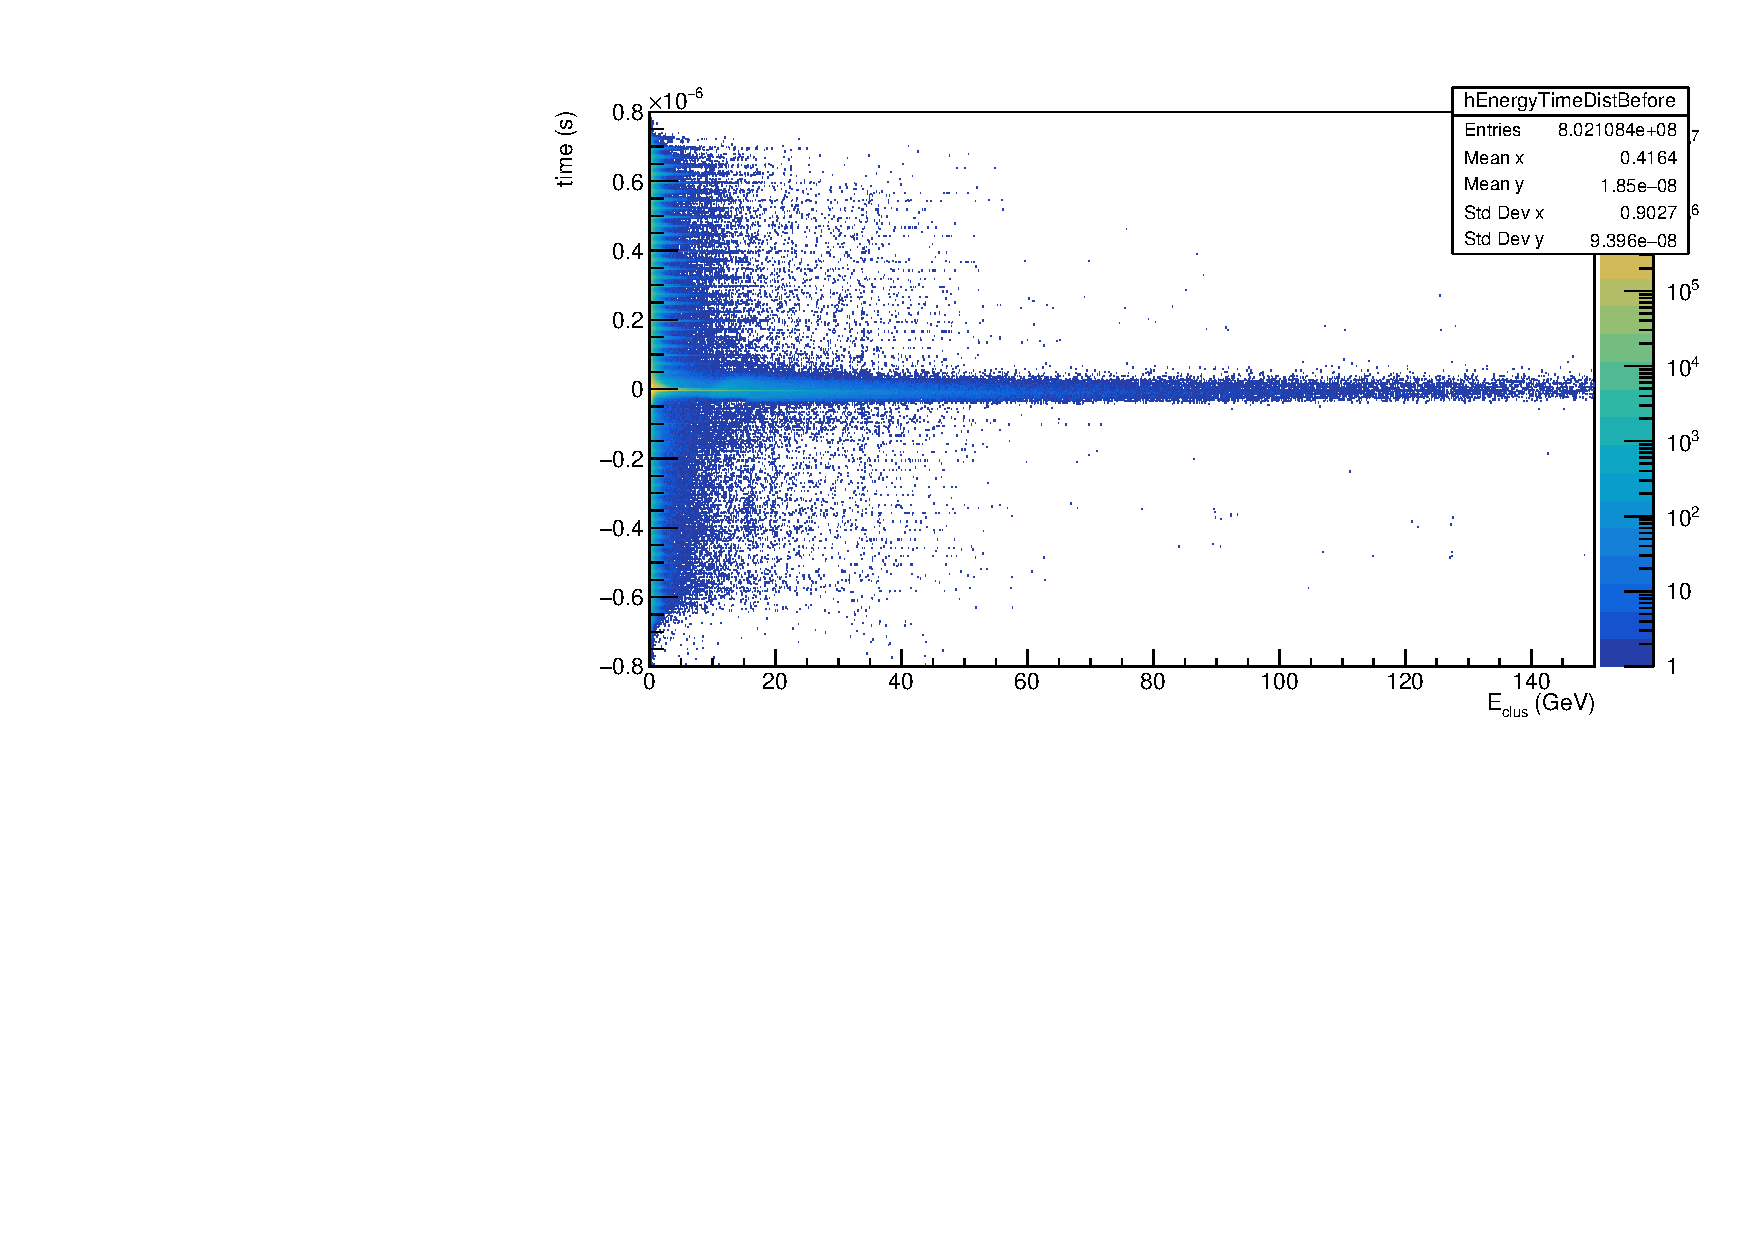
\includegraphics[width=11cm]{timming}
\centering
\caption{EMCal cluster time distribution before cuts.}
\label{fig:EMCaltime}
\end{figure}


Cutting on the cluster time is done in order to readout only the particles created from an event and to limit the contamination due to slower particles from previous events.  The main source of the slow moving particles are neutrons and $K_{L}^{0}$ and this analysis limited cluster time to $t_{clus} \, \epsilon \,$ [-50 ns, 100 ns].


\begin{figure}[h]
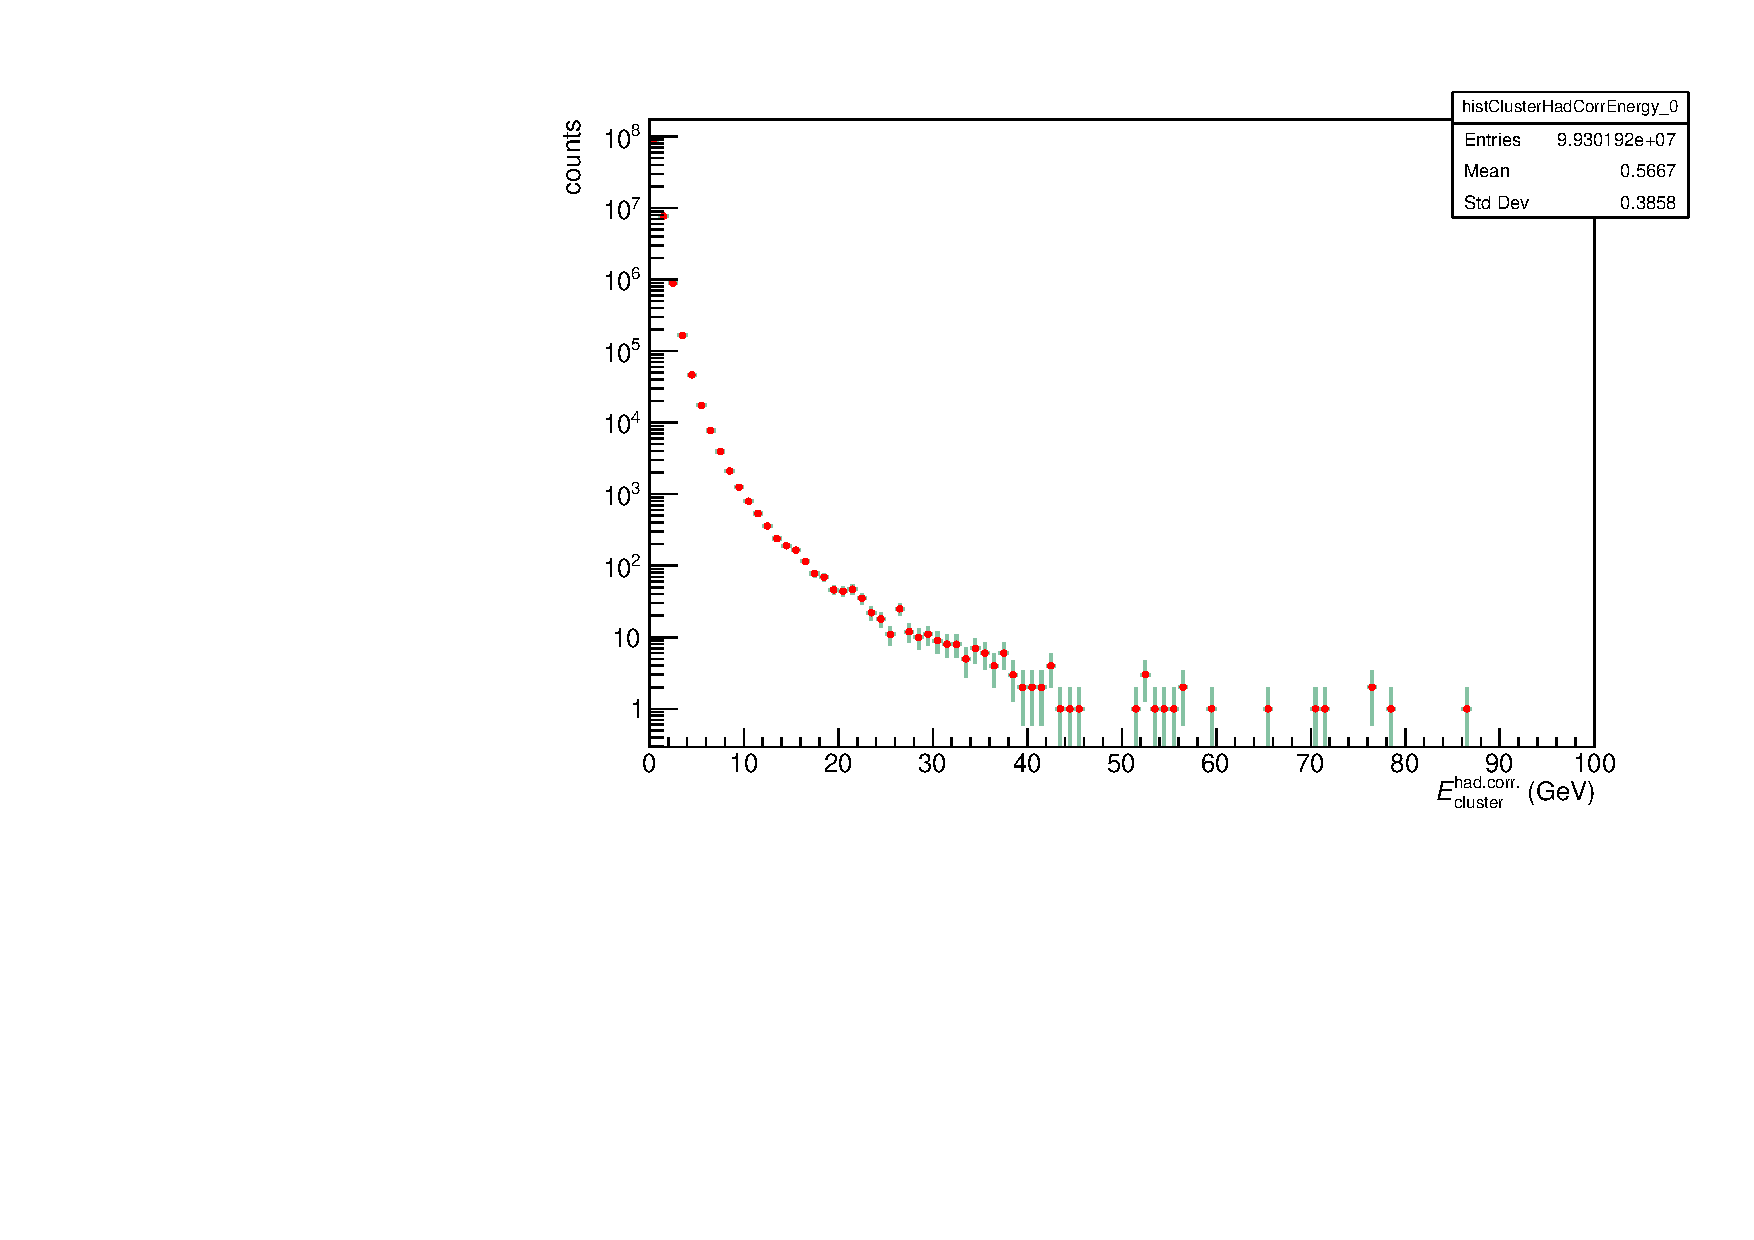
\includegraphics[width=8cm]{Eclusfinal}
\centering
\caption{Corrected EMCal cluster yield.}
\label{fig:EMCalfinal}
\end{figure}
\newpage

Figure \ref{fig:EMCalfinal} shows the final cluster energy distribution with all the cuts and corrections previously discussed applied, and makes up the set of clusters over which the jet finding was performed.  The same cuts and corrections were applied to the EMCal triggered data.

\section{Track Selection}

Tracks were reconstructed in the TPC using a Kalman filtering which helps alleviate any corrections needed due to multiple scatterings, dead sectors, etc.  Jet finding was performed using `hybrid' tracks.  Hybrid tracks consist of two track sets, the first being all tracks with at least one hit in the SPD (Global), and the second set being all tracks that can be constrained to the primary vertex (Complimentary).  The reconstruction of a signal from the ITS and TPC form good tracks if the $\chi^{2}/NDF$, chi-square per degrees of freedom, is required to be less than 4 in the TPC and $\chi^{2}$ is required to be less than 36 in the ITS. For this analysis, the minimal $p_{T, track}$ was 150 MeV/c and the track was constrained to the TPC acceptance: - 0.9 $\leq \eta \leq$ 0.9 and 0 $\leq \phi \leq$ 2$\pi$, shown in Figure \ref{fig:Hybridtracketaphi}.  The spatial distributions of the hybrid tracks remain relatively flat as expected in the 8 TeV data set for good and semi-good runs.

\begin{figure}%
    \centering
    \subfloat[Hybrid Track $\eta$]{{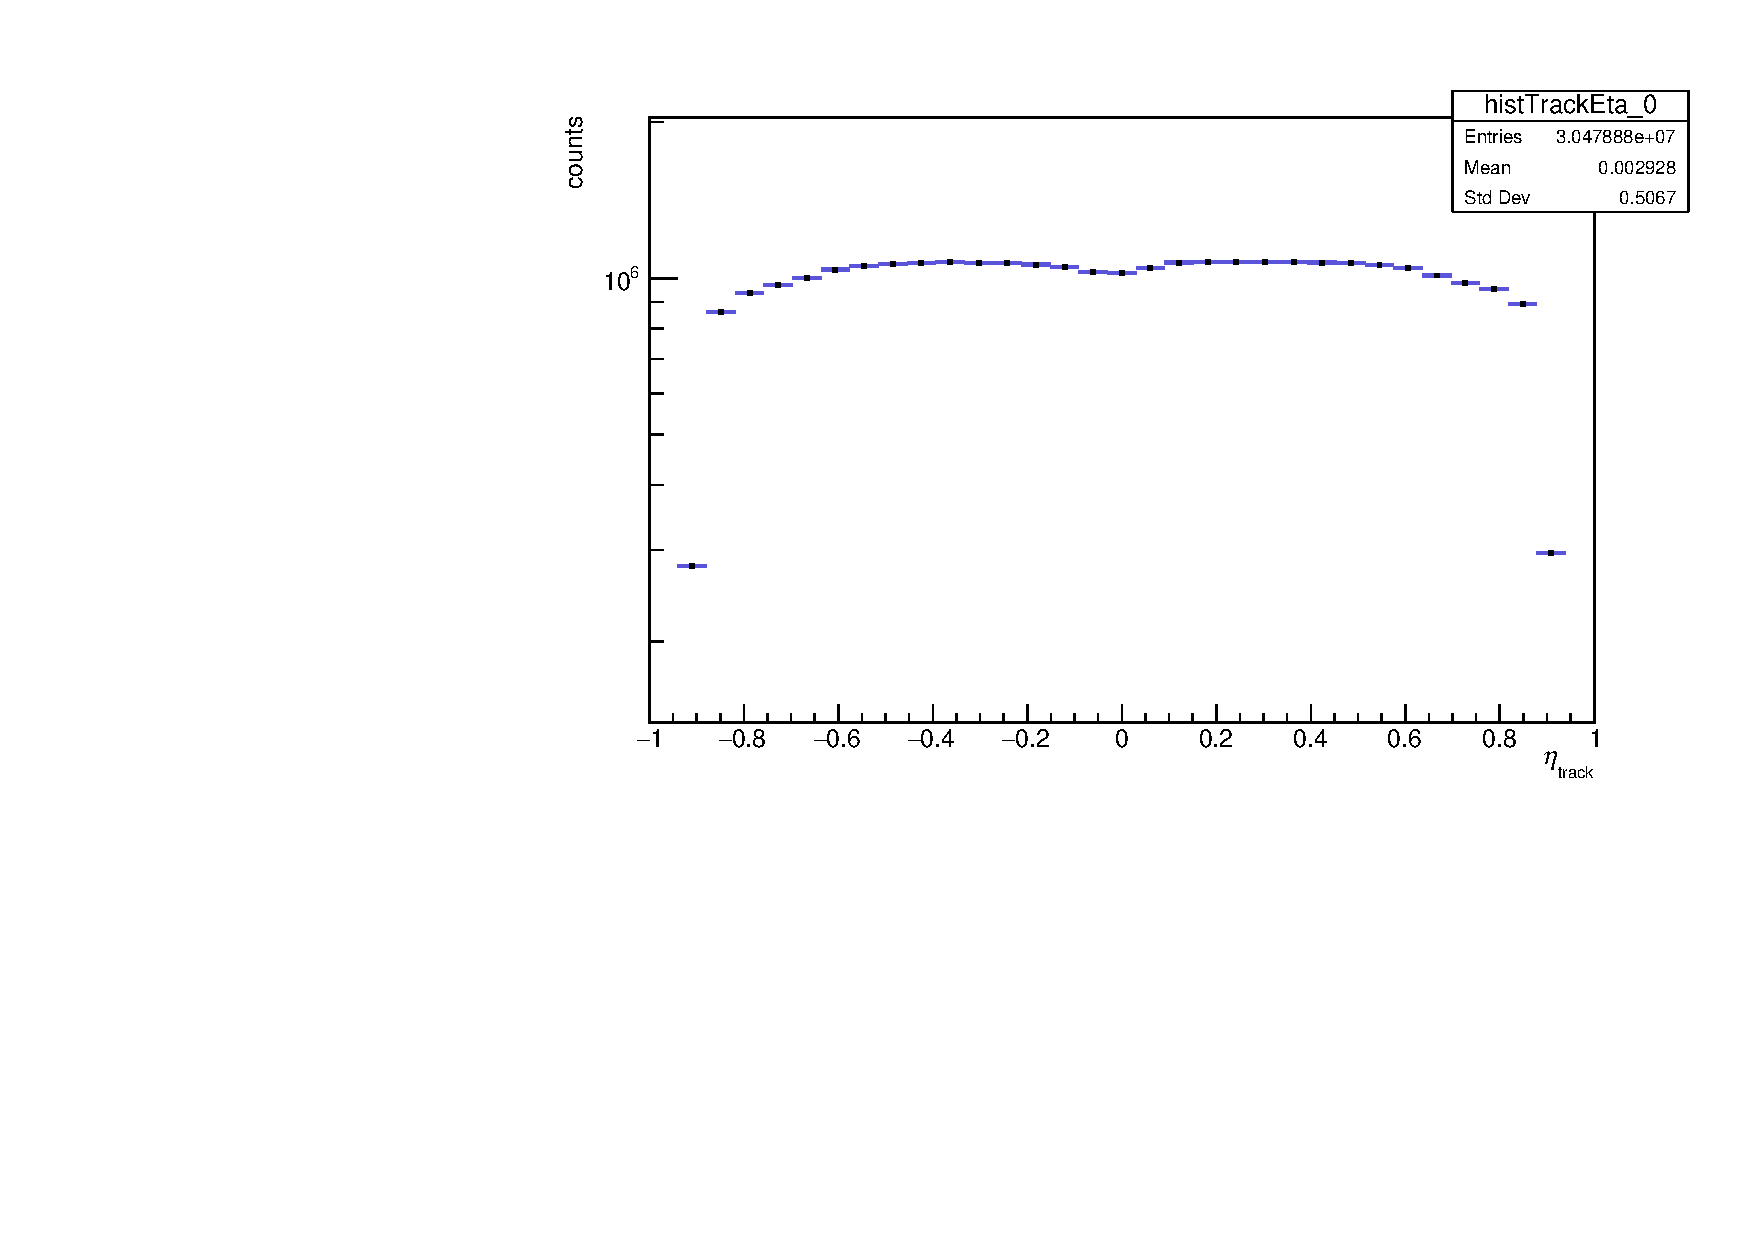
\includegraphics[width=0.4\textwidth]{tracketa} }}%
    \qquad
    \subfloat[Hybrid Track $\phi$]{{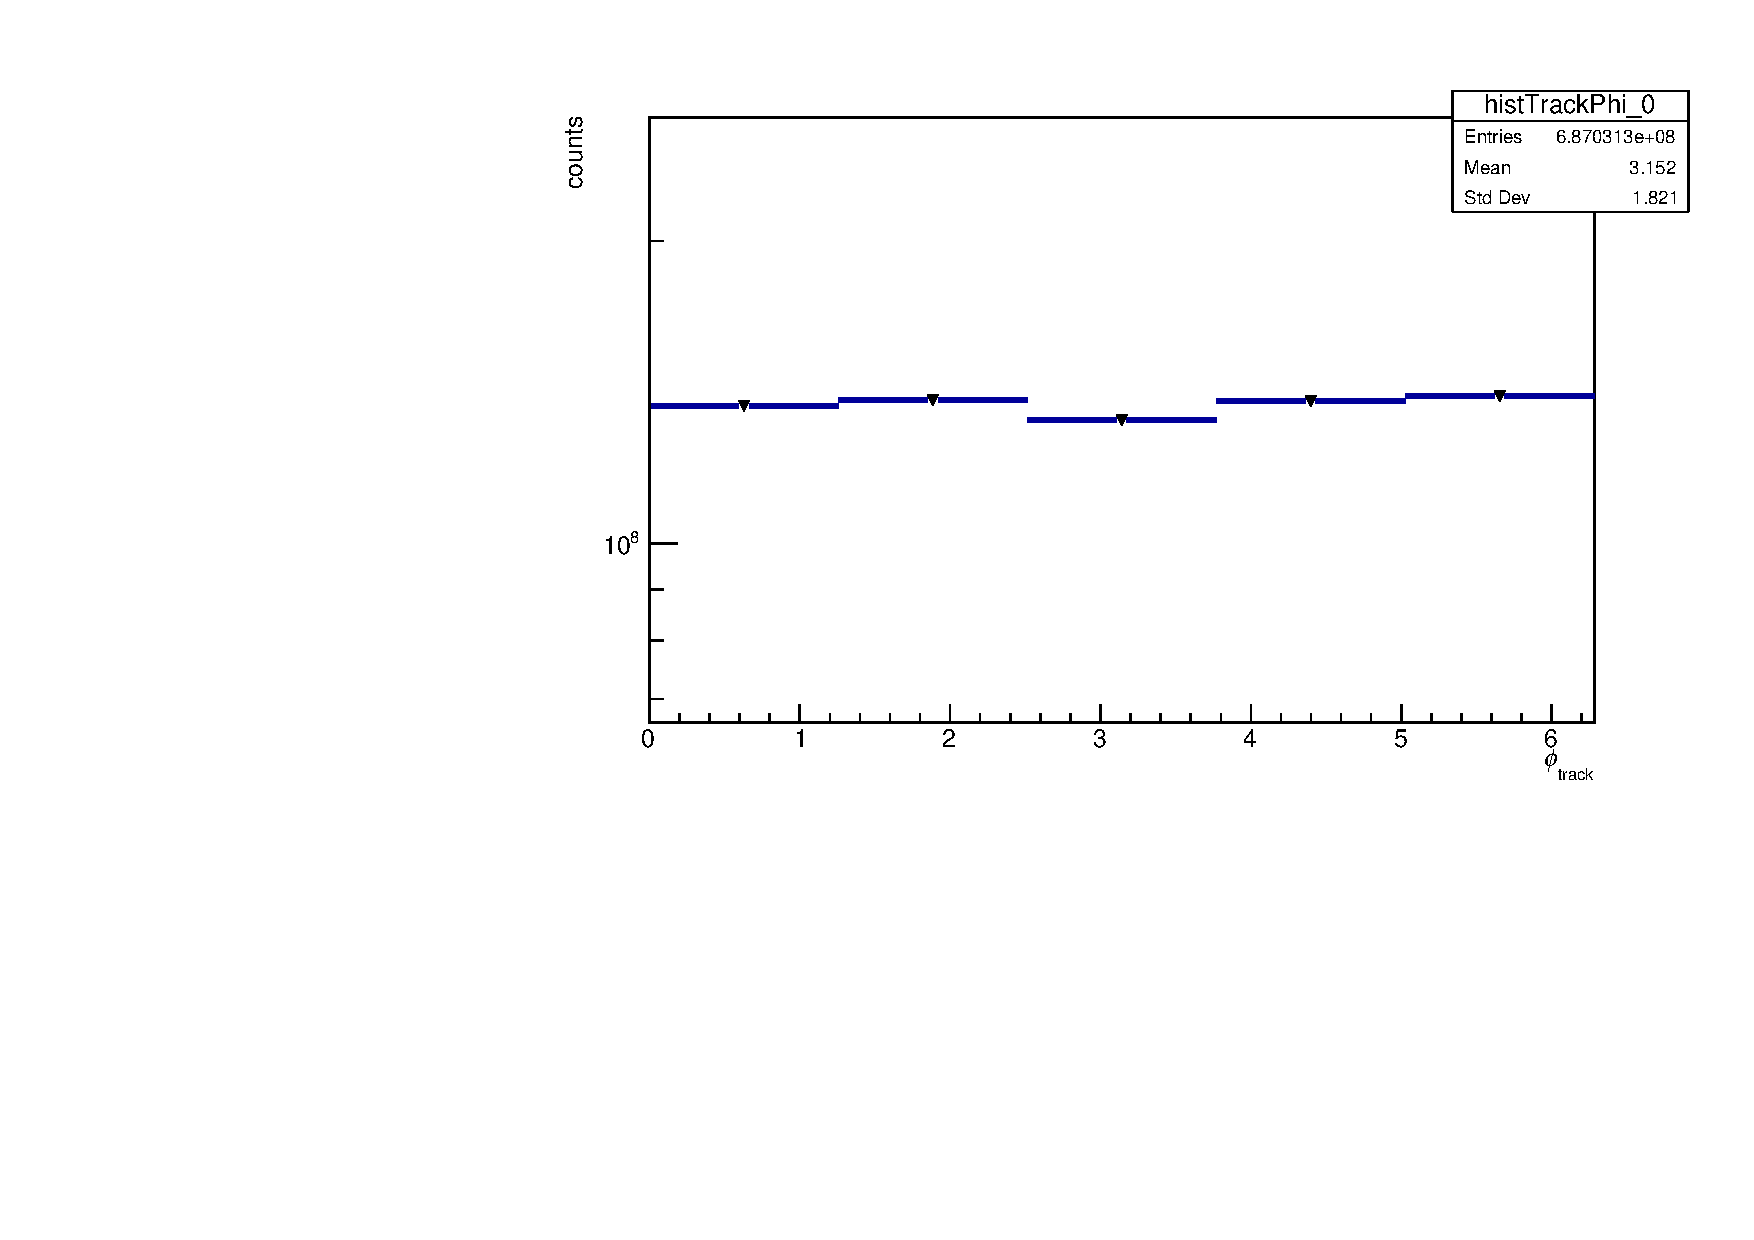
\includegraphics[width=0.4\textwidth]{trackphi} }}%
    \caption{Hybrid Track $\eta$ and $\phi$ yields.}%
    \label{fig:Hybridtracketaphi}%
\end{figure}


The quality of the jet $p_{T}$ resolution was maintained by only accepting jets into the jet finder with a resolution below 1\% as seen in Figure \ref{fig:trackresolution}, and this $p_{T}$ distribution may be seen in Figure \ref{fig:hybtrackpt}.  Tracks should travel in a smooth curve unless they decay in the detector.  Some tracks in the TPC exhibit a kink due to the particle decaying.  Due to complications that would arise from trying to include these tracks in jet finding, any track with a kink was excluded from this analysis.  These cuts followed a number of previous track cuts seen in a number of jet results published from ALICE\cite{Acharya:2018eat}.

\begin{figure}[h]
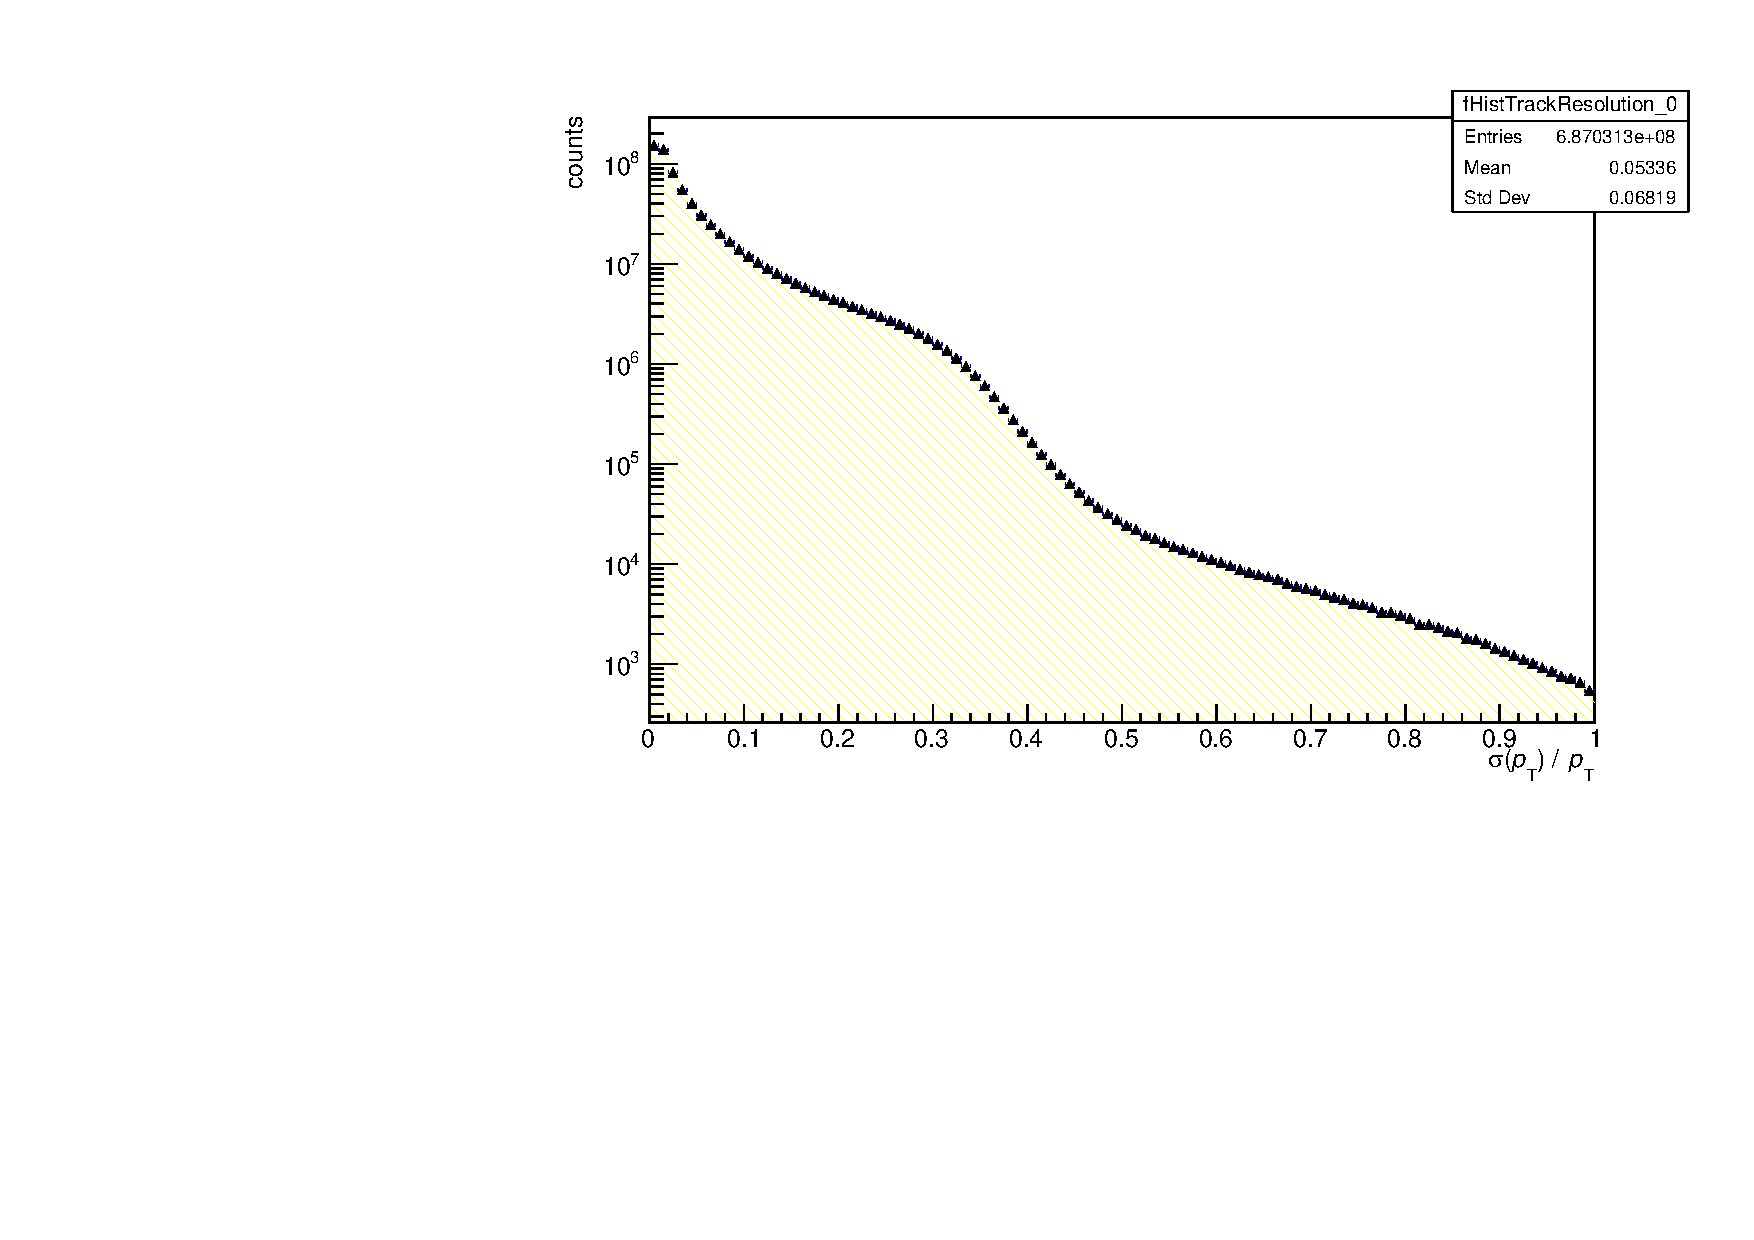
\includegraphics[width=8cm]{trackresolution}
\centering
\caption{Accepted hybrid track resolution.}
\label{fig:trackresolution}
\end{figure}

\begin{figure}[h]
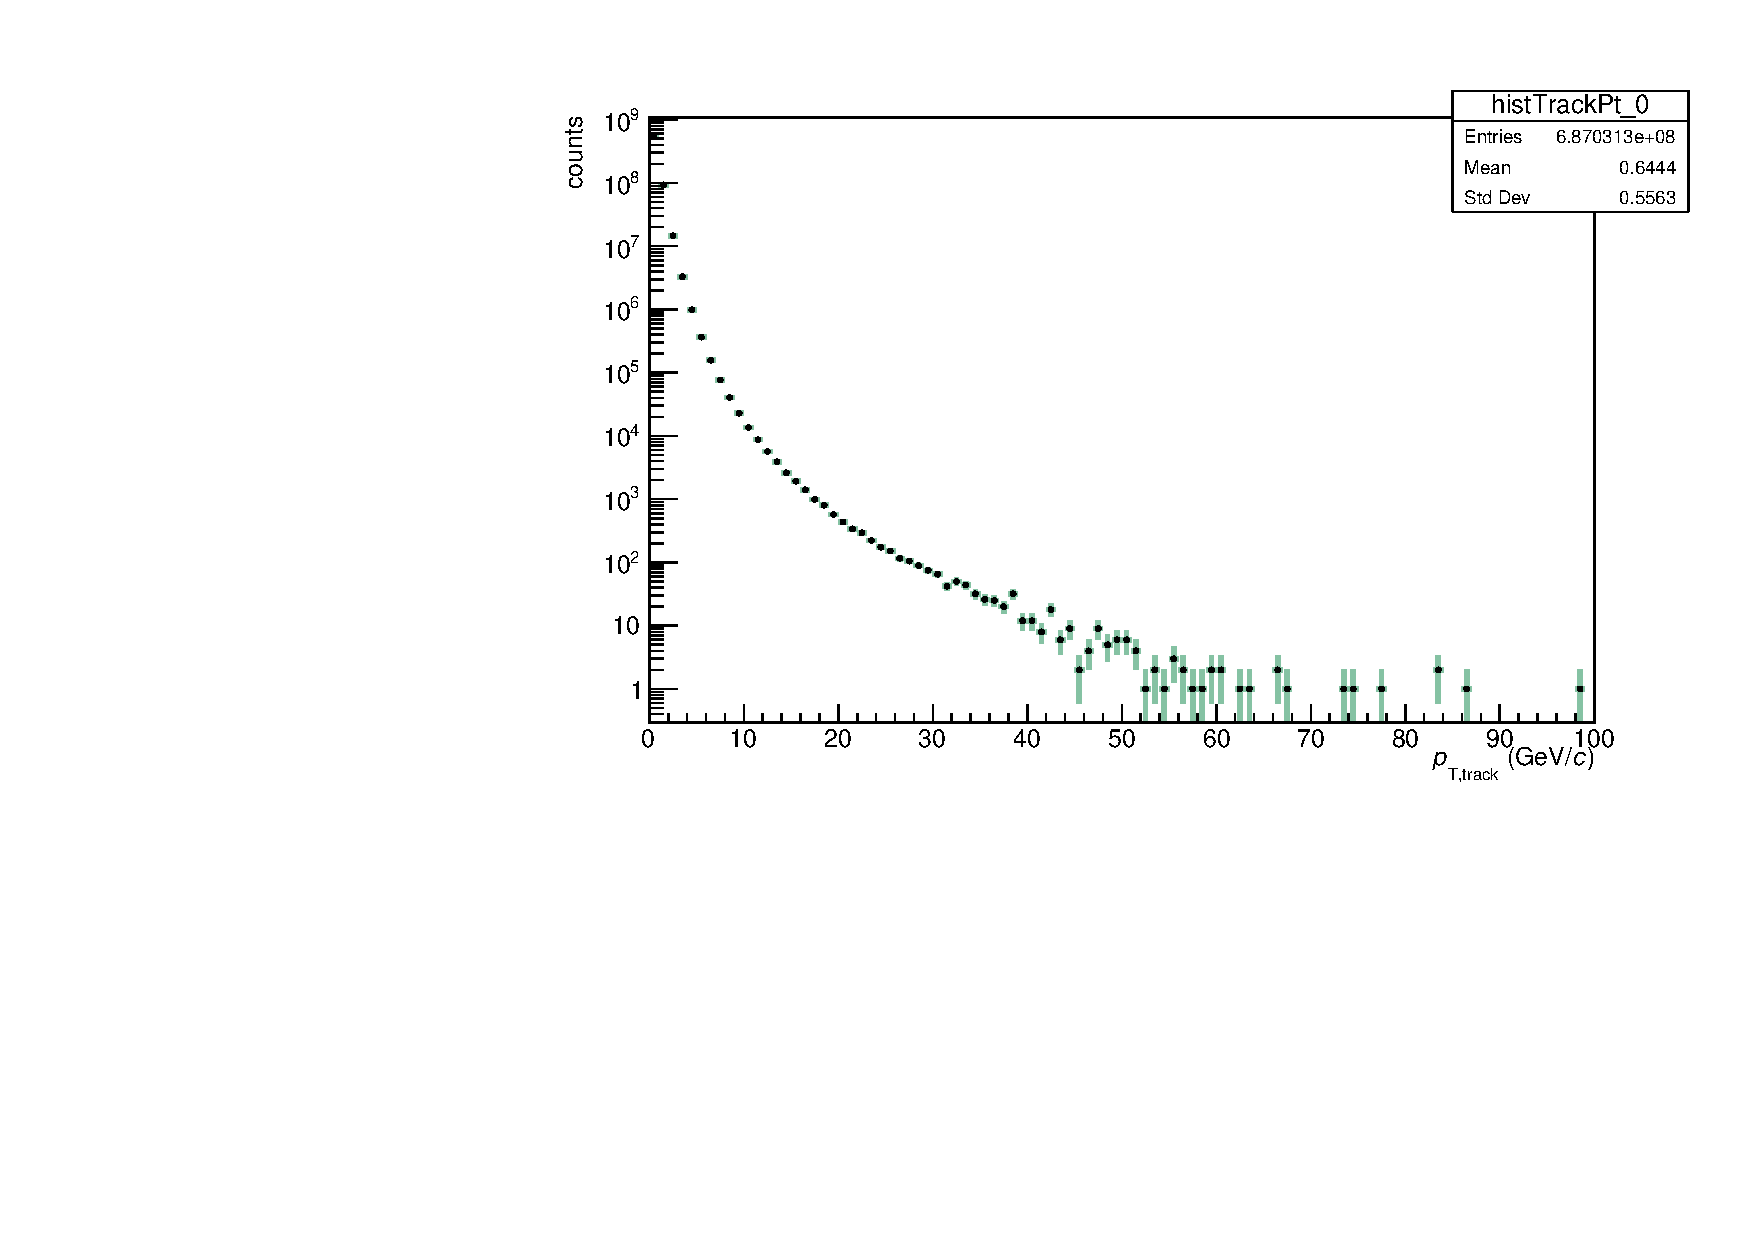
\includegraphics[width=8cm]{trackpt}
\centering
\caption{Accepted track $p_{T}$ yield.}
\label{fig:hybtrackpt}
\end{figure}


\section{Jet Selection}

Accepted tracks and clusters were pipped into the anti-kt jet reconstruction algorithm to measure inclusive jets.  A minimum threshold of 5 GeV was used to reconstruct a jet in this analysis.  A high-$p_{T}$ track threshold of 100 GeV was placed on the reconstructed jets.  This was motivated by the degradation of the momentum resolution above that energy range.  In addition a cut was applied that a jet must be composed of at least one constituent, as shown in Figure \ref{fig:JetPt} and \ref{fig:JetConst}.

\begin{figure}[h]
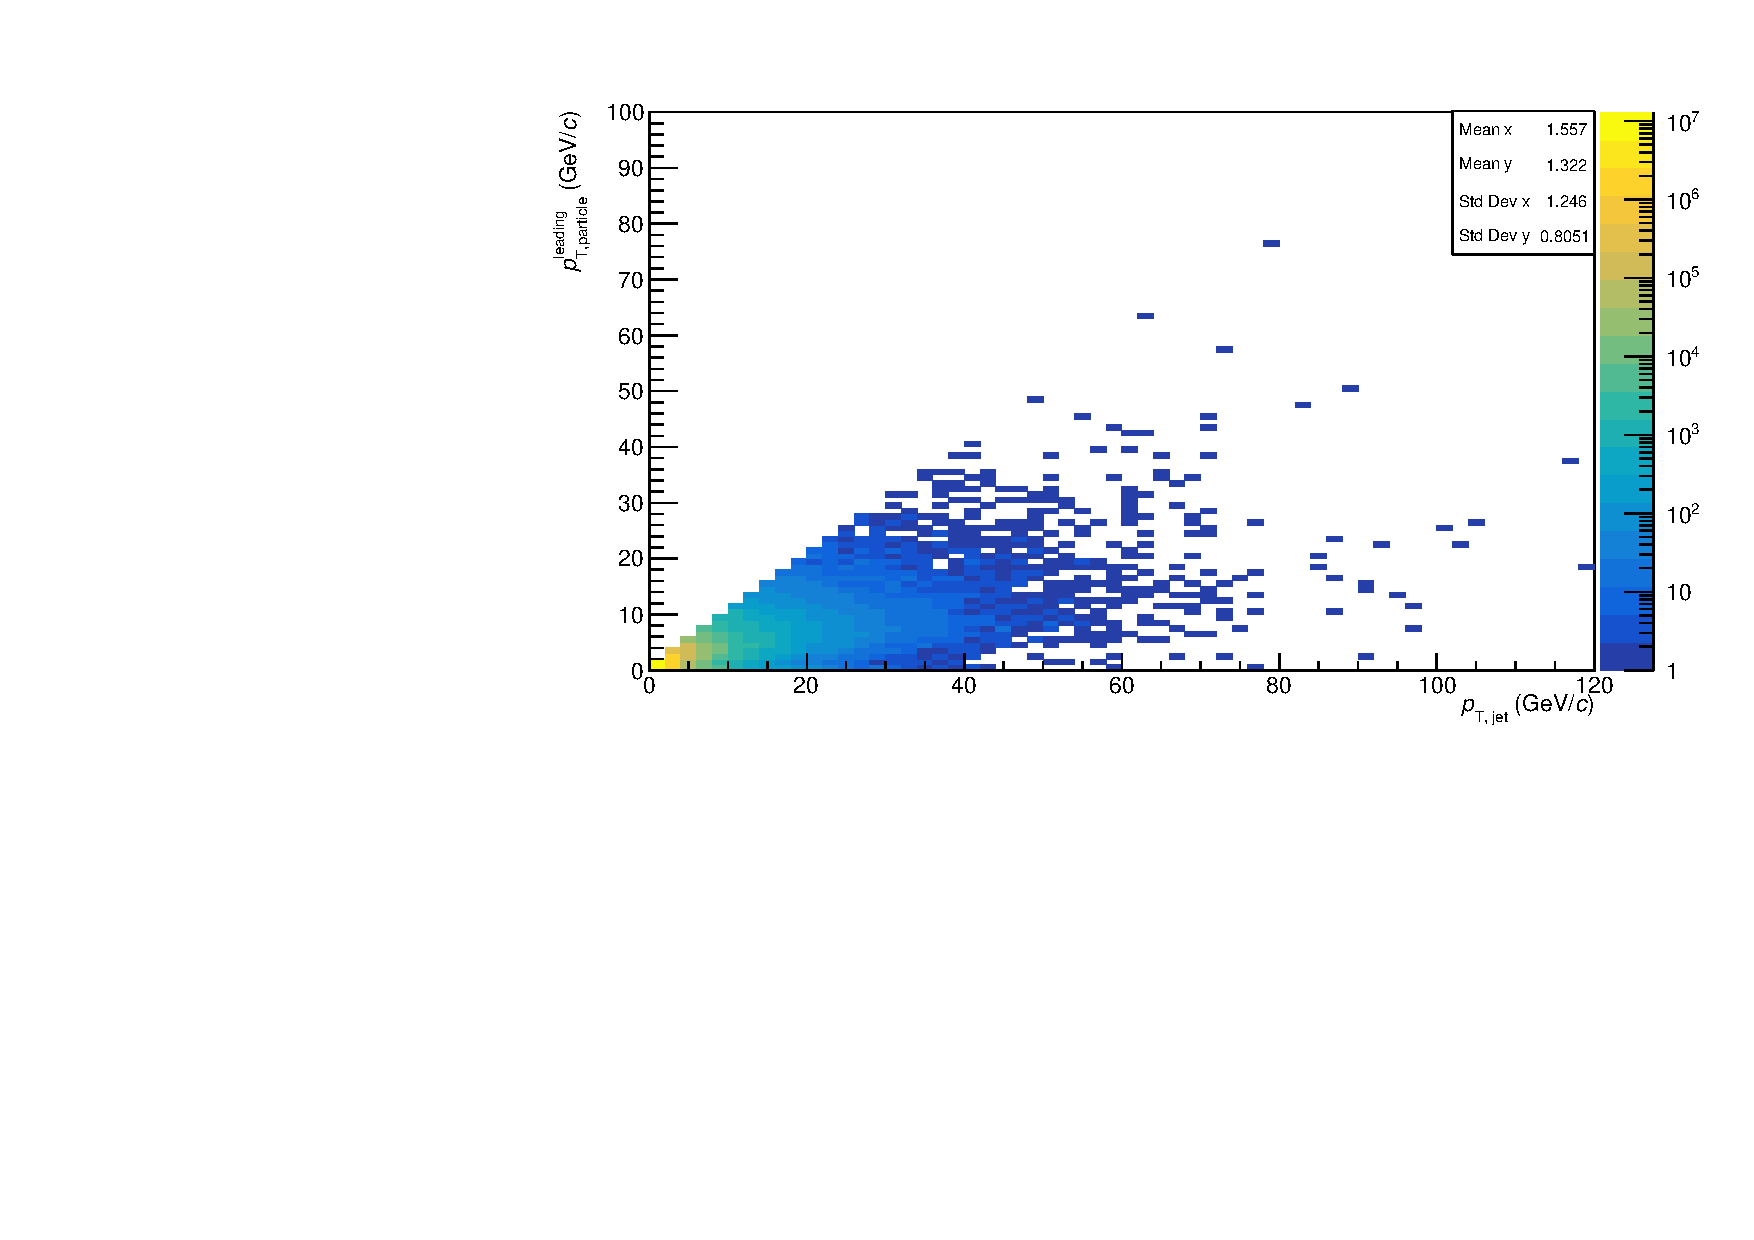
\includegraphics[width=8cm]{ptleadingR02}
\centering
\caption{R = 0.2 leading track $p_{T}$ per jet $p_{T}$.}
\label{fig:JetPt}
\end{figure}

\begin{figure}[h]
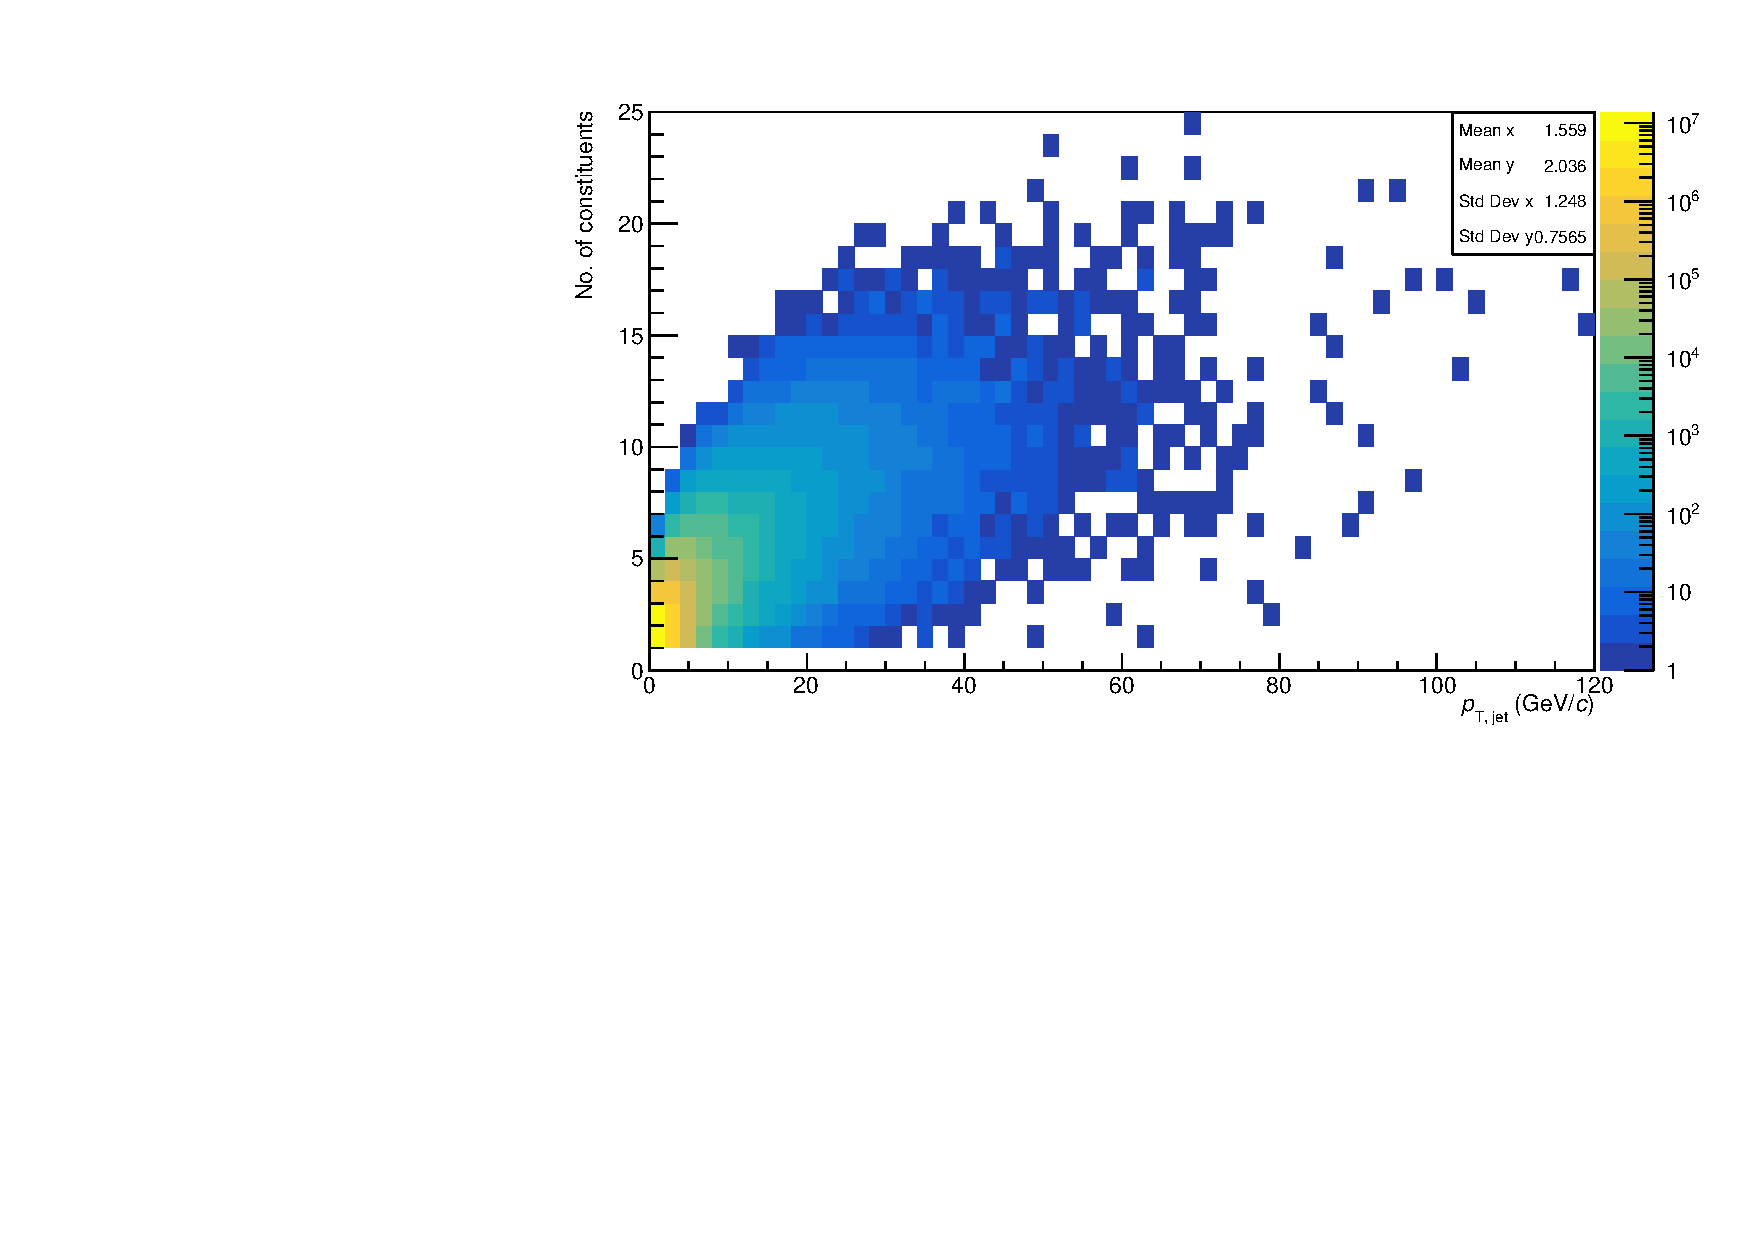
\includegraphics[width=8cm]{JetnumcconstR02}
\centering
\caption{R = 0.2 number of constituents in a jet per jet $p_{T}$.}
\label{fig:JetConst}
\end{figure}



The fragmentation function for the leading track in a jet,

\begin{equation}
z_{leading} = \frac{ p_{leading, proj} }{ p_{jet} },
\label{eq:zleading}
\end{equation}

\noindent
may be artificially high due to misidentifying secondary decay particles as primary vertex tracks and assigning them a much larger $p_{T}$.  Additionally, fake clusters, such as exotics, may skew the jet $p_{T}$ to apparently large values and thus make $z_{leading}$ infinitesimal.  

\begin{figure}[h]
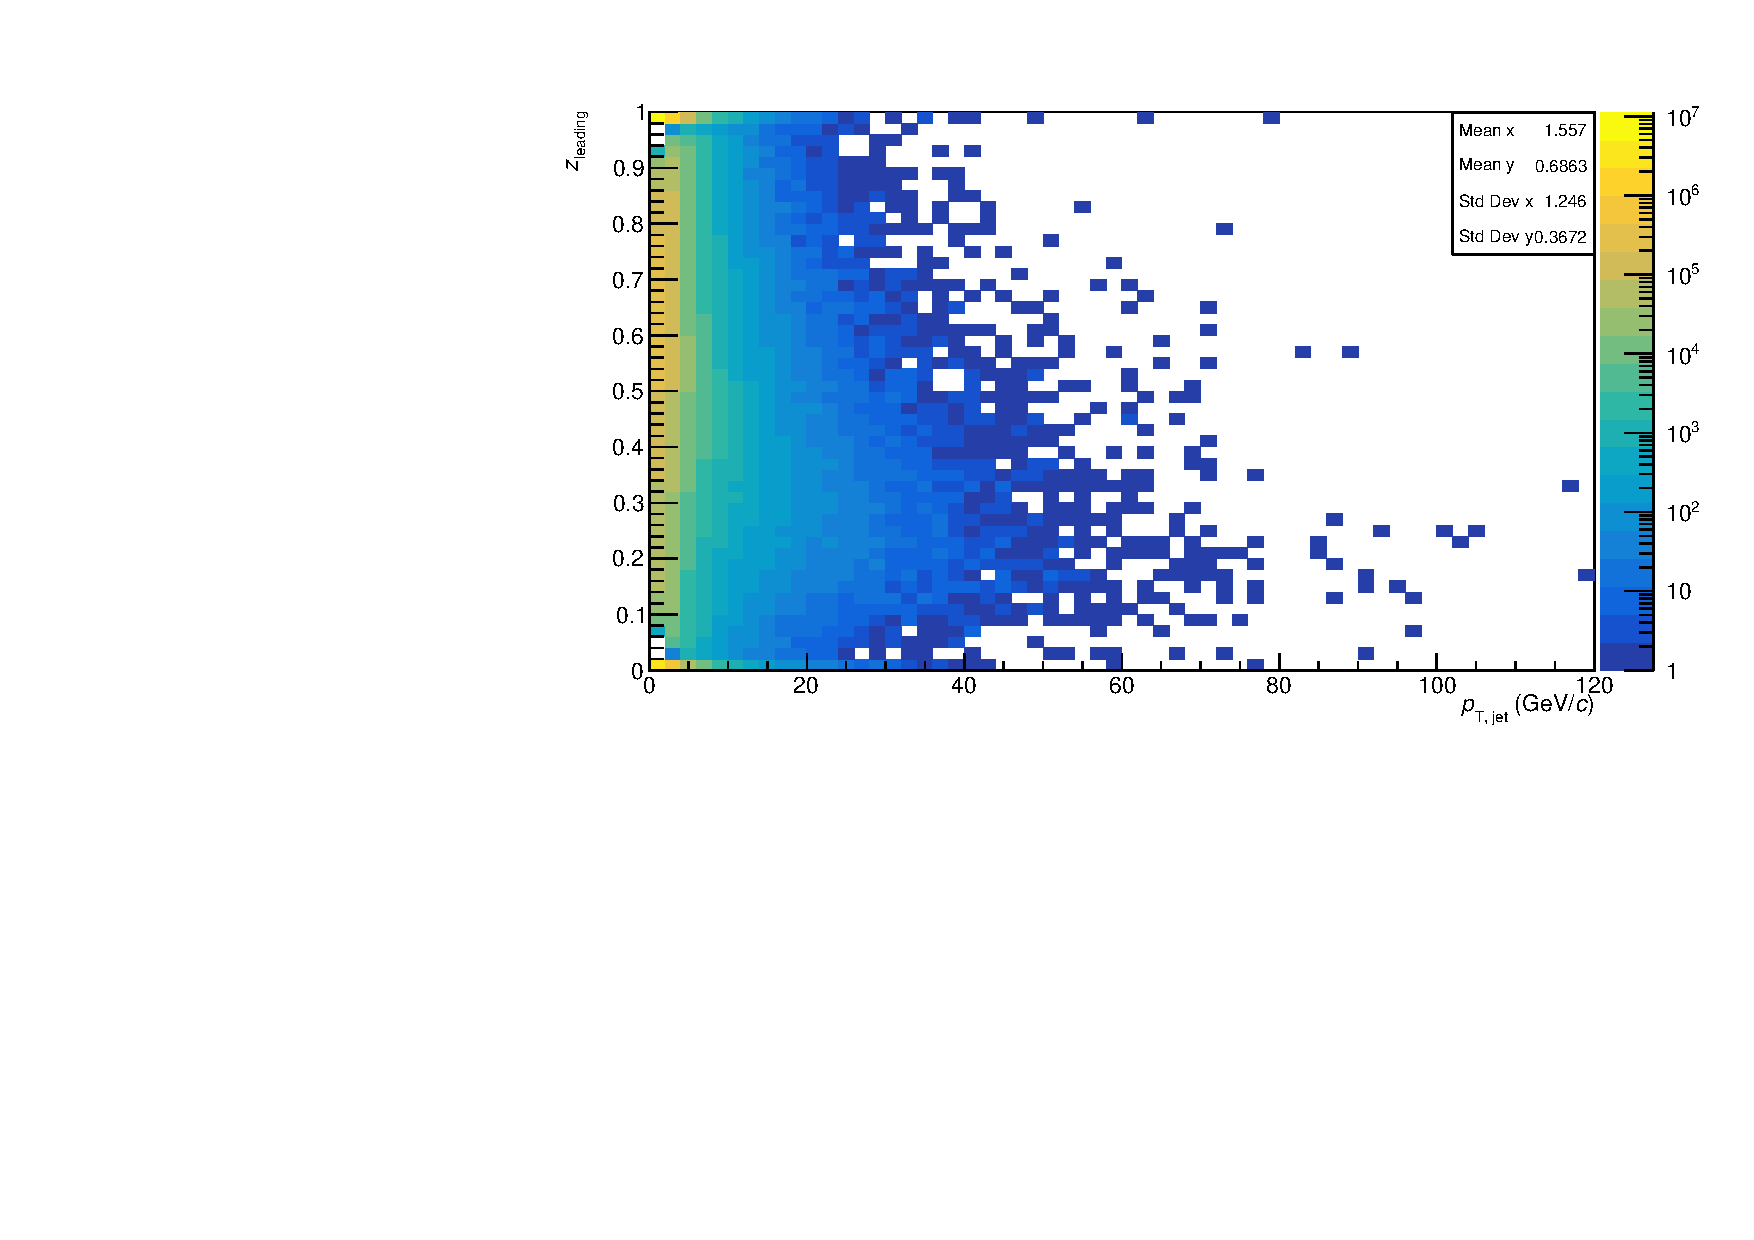
\includegraphics[width=10cm]{JetzR02}
\centering
\caption{R = 0.2 $z_{leading}$ from the Min Bias data sample.}
\label{fig:Jetz}
\end{figure}

Figure \ref{fig:Jetz} shows the projection of the hadronic 3-momentum onto the jet axis.  We observed an excess of jets, especially at low jet $p_{T}$, of z values close to 1 or zero.  Previous jet results from ALICE removed these biased jets with a cut on $ z_{leading} \geq 0.03$ and $z_{leading} \leq 0.97$ is imposed.  It should also be noted that due to QCD hadronization $z_{leading} \sim 1$ corresponds to a jet dominated by a singular high-$p_{T}$ particle, howver this is allowed by QCD and thus no $z_{leading}$ cut was implemented in this analysis.  In between .03 and .97 we see the $z_{leading}$ is continuous and uniform as expected.  

A jet area of, $A_{jet}$, cut was imposed on accepted jets.

\begin{equation}
A_{jet} \geq 0.6 \pi R_{jet}^{2}
\label{eq:AreaJet}
\end{equation}

The area is estimated in FastJet using `ghost' particles.  As jet reconstruction is being performed, these fake particles with infinitesimal $p_{T}$ are placed randomly throughout the event.  The number of ghost particles captured in a jet is proportional to the jet area, thus the precision of the jet area is sensative to the reconstruction of soft particles.  Figure \ref{fig:jetRejection} shows the rejection reason for a jet with the dominate reasoning due to the area cut, this cut skewed towards low-$p_{T}$ jets.

\begin{figure}[h]
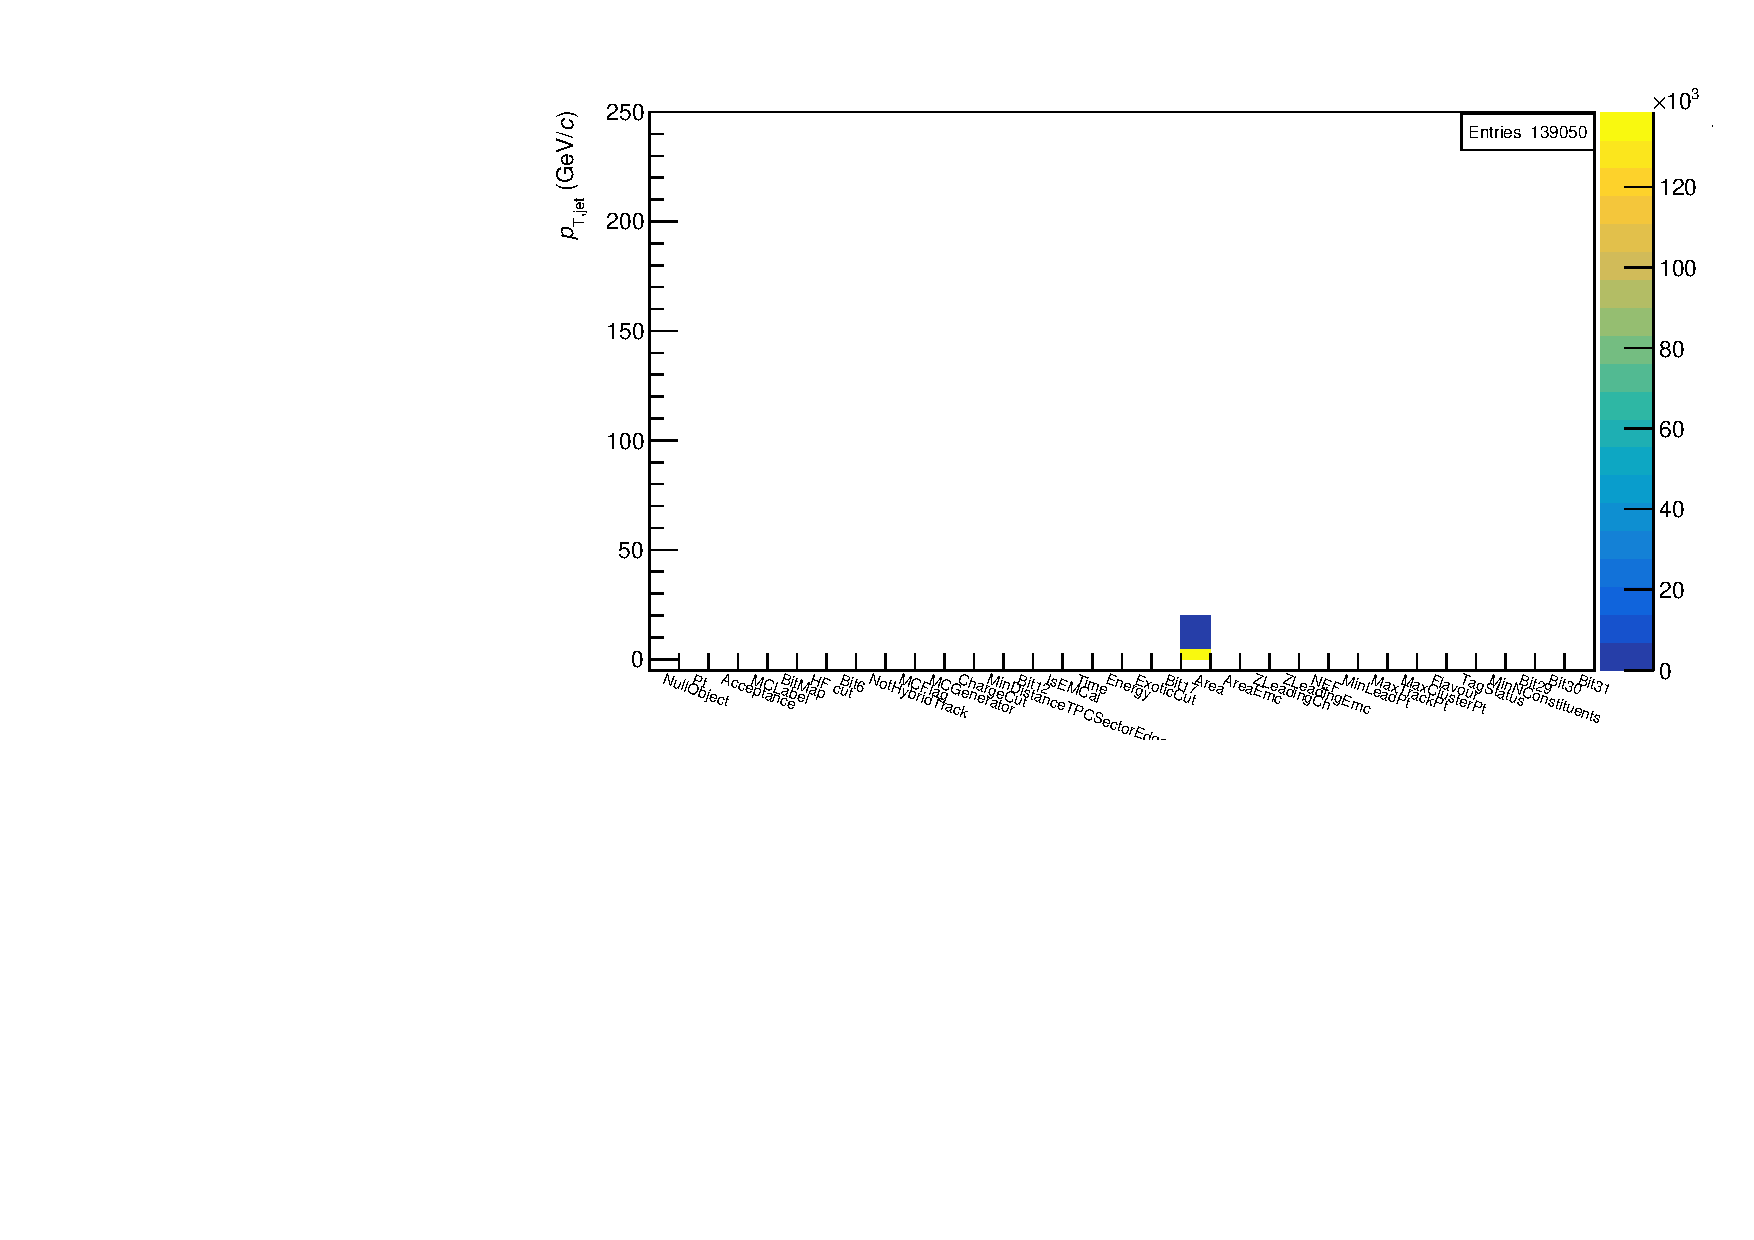
\includegraphics[width=12cm]{jetRejection}
\centering
\caption{Jet rejection reason.}
\label{fig:jetRejection}
\end{figure}


The Neutral Energy Fraction (NEF) is the total jet energy carried by the neutral components of the jet, i.e. EMCal clusters.  Figure \ref{fig:JetNEF} shows the NEF for R = 0.2 jets from the Min Bias sample.


We observed an excess of jets at low-$p_{T}$ with NEF values around zero or one, similar to what was seen with the $z_{leading}$ distribution.  The cause for these excesses were explored in this analysis, but no hard source was identified and no cut to the NEF was used.  Because this is not a well understood pheonmena no NEF cut was implemented, but this is something that should be explored in future analysis.


After this exploratory data analysis was performed and the cuts that were used were implemented I obtained my sample of the signal jets that are reported in the cross section and spectra.  These criteria were implemented for the R = 0.3 and R = 0.4 along with the EMCal triggered data.

\begin{figure}[h]
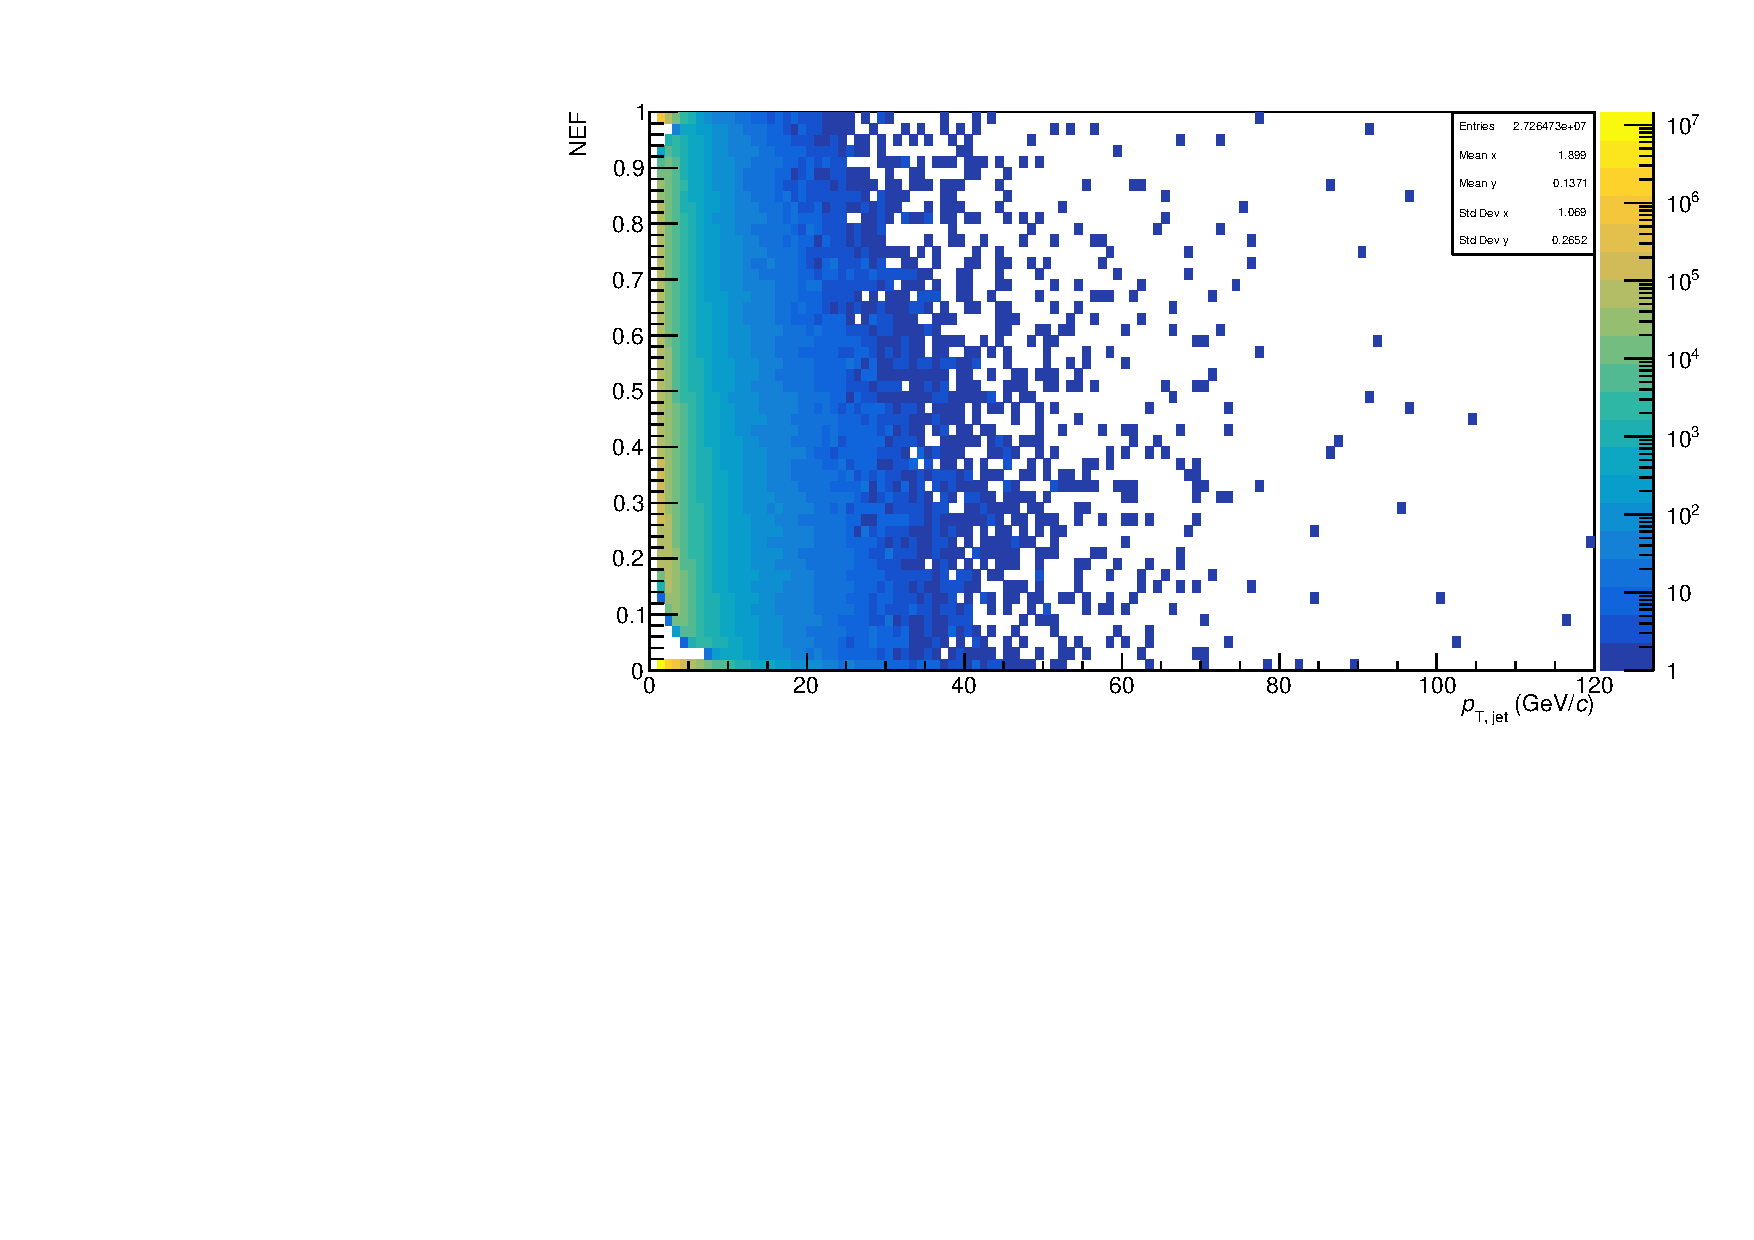
\includegraphics[width=10cm]{NEFR02}
\centering
\caption{R = 0.2 NEF per jet $P_{T}$.}
\label{fig:JetNEF}
\end{figure}




